%% Ejemplo de la plantilla de latex para las diapositivas del Máster en IA 

%%%%%%%%%%%%%%%%%%%%%%%%%%%%
%% Valores para el ratio de aspecto: 43, 169 
%\documentclass[10pt, envcountsect, presentation, aspectratio=1610, hyperref={hypertexnames=true}]{beamer}
\documentclass[10pt, envcountsect, handout, aspectratio=1610, hyperref={hypertexnames=true}]{beamer}

%%%%%%%%%%%%%%%%%%%%%%%%%%%%

%%%%%%%%%%%%%%%%%%%%%%%%%%%%
%% Incluir fichero de estilo del máster
\input ../style/plantillaMasterIA.sty
%%%%%%%%%%%%%%%%%%%%%%%%%%%%

\addbibresource{../references.bib}



%\setbeameroption{show only notes} % Only notes
%\setbeameroption{show notes on second screen=right}  % Both
%\setbeamertemplate{note page}[compress]
\setbeameroption{hide notes} % Only slides



\renewcommand*\footnoterule{}
\setbeamerfont{footnote}{size=\tiny}




%\input{embed_video.tex}
%\usepackage{movie15}
\usepackage{multimedia}


%%%%%%%%%%%%%%%%%%%%%%%%%%%%
%% Información que aparecerá en la portada
\title[Aprendizaje por Refuerzo]{Aprendizaje por Refuerzo}
\subtitle{Proceso de Decisión de Markov} % short title for footer

\author[L. D. Hernández] % Para el pie de página, poner los autores abreviados separados por comas.
{%
	\sc{Luis Daniel Hernández Molinero }\\ % Autor 1
	\textit{Ciencia de la Computación e Inteligencia Artificial}\\  % Area de conocimiento
	\textit{Dept. Ingeniería de la Información y las Comunicaciones}\\  % Departamento
	\\   % No dejes espacio entre esta línea y la llave siguiente 
}

\institute[DIIC]% % Poner las iniciales de los diferentes departamentos de los autores separadas por comas.
{
	\textit{Universidad de Murcia}
}

\newcounter{yearnext}
\setcounter{yearnext}{\the\year}
\addtocounter{yearnext}{-1}

\date{\arabic{yearnext} / \the\year\ } % Curso académico

%%%%%%%%%%%%%%%%%%%%%%%%%%%%%%%%%%
%% Contenido de las diapositivas
\setbeamerfont{normal text}{size=\normalsize} % Modifica el tamaño del texto de las diapositivas.
\AtBeginDocument{\usebeamerfont{normal text}}

%%%%%%%%%%%%%%%%%%%%%%%%%%%%%%%%%%

\begin{document}	

%%%%%%%%%%%%%%%%%%%%%%%%%%%%%%%%%%









%%%%%%%%%%%%%%%%%%%%%%%%%%%%%%%%%%

\begin{frame}[plain]
	\titlepage
\end{frame}

%%%%%%%%%%%%%%%%%%%%%%%%%%%%%%%%%%

\begin{frame}{Índice de Contenidos}
	\tableofcontents 
\end{frame}



%%%%%%%%%%%%%%%%%%%%%%%%%%%%%%%%%%
%%%%%%%%%%%%%%%%%%%%%%%%%%%%%%%%%%
\section{Introducción a los Procesos Estocásticos}


%%%%%%%%%%%%%%%%%%%%%%%%%%%%%%%%%%
%%%%%%%%%%%%%%%%%%%%%%%%%%%%%%%%%%
\begin{frame}{Introducción}
\begin{itemize}
\item Un \key{sistema} es un conjunto de elementos interrelacionados que funcionan como un todo para lograr un objetivo común.

    \unEjemplo Un automóvil, un reloj, una célula, etc ...
\hfil
\begin{tikzpicture}[scale=0.5, baseline]

    % Dibujar la caja negra con texto blanco
    \node[rectangle, fill=black, text=white, minimum width=1.5cm, minimum height=1cm, align=center] (caja) 
    {\textbf{\scriptsize Caja} \\ \textbf{\scriptsize Negra}};
    
    % Flecha de entrada a la izquierda de la caja
    \draw[->, thick] 
        ($(caja.west) + (-2cm, 0)$) -- (caja.west)
        node[midway, above] {\scriptsize Entrada};
    
    % Flecha de salida a la derecha de la caja
    \draw[->, thick] 
        (caja.east) -- ($(caja.east) + (2cm, 0)$)
        node[midway, above] {\scriptsize Salida};

\end{tikzpicture}


\item Muchos sistemas evolucionan a lo largo del \key{tiempo} y  presentan las siguientes características:

\begin{itemize}
\item Existe \key{incertidumbre}: El futuro no está completamente determinado por el presente.

\item Hay \key{aleatoriedad}: Los eventos ocurren de forma aleatoria, siguiendo ciertas distribuciones de probabilidad.

\item La información es \key{incompleta}: No se conoce toda la información necesaria para hacer predicciones exactas.

\end{itemize}

\unEjemplo Finanzas, meteorología, comunicaciones, bilogía, física, etc\\

\item ¿Cómo estudiar estos sistemas?

\begin{itemize}
\item \key[red]{Objetivo:} Establecer una representación matemática (modelo) del fenómeno (sistema). 

\item \key{Solución:} Procesos estocásticos 
\end{itemize}
\end{itemize}

%son herramientas fundamentales en diversas áreas de la ciencia y la ingeniería porque nos permiten modelar y analizar fenómenos que presentan un componente aleatorio o incierto. En esencia, nos ayudan a comprender y predecir sistemas que evolucionan en el tiempo de manera no determinista.
\end{frame}




%%%%%%%%%%%%%%%%%%%%%%%%%%%%%%%%%%
%%%%%%%%%%%%%%%%%%%%%%%%%%%%%%%%%%
\subsection{Variables Aleatorias y sus Distribuciones de Probabilidad}

%%%%%%%%%%%%%%%%%%%%%%%%%%%%%%%%%%
%%%%%%%%%%%%%%%%%%%%%%%%%%%%%%%%%%
\begin{frame}{Variable Aleatoria}
\begin{definition}
\begin{itemize}
    \item Una \key{variable aleatoria} es una función desde un espacio muestral $\Omega$ en $\mathbb{R}$.
    \item Un \key{espacio muestral} es el conjunto de los posibles \textbf{resultados} de un experimento, llamados sucesos elementales.
    \item La variable aleatoria asigna a $w \in \Omega$ un número real $X(w)$, de forma \key{atemporal}.
    \item Podemos extender el concepto a variable aleatoria \key{cualitativa}.
\end{itemize}
\end{definition}

\small
\begin{example}[Lanzamiento de dos monedas]
\begin{itemize}
    \item Experimento: Lanzar dos monedas al aire.
    \item Espacio muestral: $\Omega = \{cc, cx, xc, xx\}$, donde $c$ representa ''sale cara'' y $x$ ''sale cruz''.
    \item Variable aleatoria $X$:
\[
\begin{array}{rcl}
X: \Omega & \longrightarrow & \mathbb{R}, \ \ \mathbb{L}abels \\
w & \mapsto & X(w) \\  
cc & \rightarrow & 2, \mbox{\ \ 2 caras} \\
cx, xc & \rightarrow & 1, \mbox{\ \ distintas} \\
xx & \rightarrow & 0, \mbox{\ \ 2 cruces} 
\end{array}
\]
\end{itemize}

\end{example}

\end{frame}



%%%%%%%%%%%%%%%%%%%%%%%%%%%%%%%%%%
%%%%%%%%%%%%%%%%%%%%%%%%%%%%%%%%%%
\begin{frame}{Distribuciones de Probabilidad con Variables Discretas}

\begin{itemize}
	\item $X: \Omega \rightarrow \mathbb{R}$ variable aleatoria \textbf{discreta} en el espacio de probabilístico $(\Omega, \mathbb{B}, Pr)$ 
	
	
\hfil $\Omega$: Espacio muestral,
		$\mathbb{B}$: $\sigma$-álgebra sobre $\Omega$,
			$Pr()$: \key{Medida de probabilidad}.

\hfil $Pr: \mathbb{B} \rightarrow [0,1]$, 
		$Pr(\emptyset)=0$, 
			$Pr(\Omega)=1$, 
				$Pr(\bigcup_{i=1}^{\infty} A_i) = \sum_{i=1}^{\infty} Pr(A_i)$
				
				
    \item Función de  \key{distribución de probabilidad} (o masa de probabilidad):\\
			\hfil $p_X(k)=P(X = k) = Pr(\{\omega \in \Omega : X(\omega) = k\})$
	
	\item Función de  \key{distribución  de probabilidad acumulada:} 
			\hfil $F_X(x) = P(X \leq x) = \sum_{k \leq x} p_X(k)$
	
	 \hfil
	 \raisebox{-0.5\height}{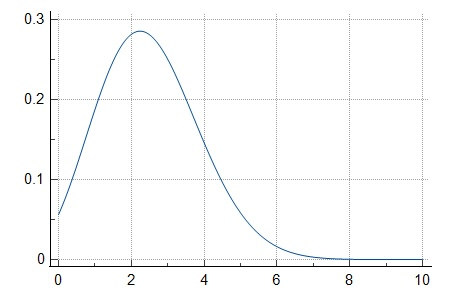
\includegraphics[width=.3\textwidth]{fig/fdp_binomial.jpg}}
	\raisebox{-0.5\height}{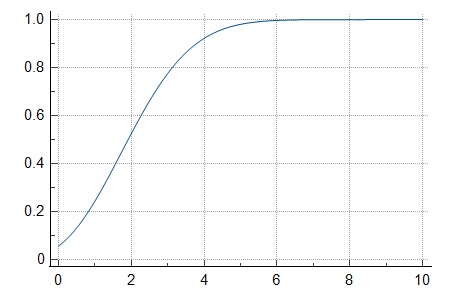
\includegraphics[width=.3\textwidth]{fig/fdpc_binomial.jpg}} 
	$\stackrel{\mbox{\tiny\url{https://www.medcalc.org/}}}{B(n=10, p=0.25)}$
	
	\item Función de  \key{distribución conjunta} y \key{d.c. acumulada} de dos variables discretas:  \\
			\hfil $P(X = x,  Y = y) = P(X = x \wedge  Y = y)$
			\hfil $F_{X, Y}(x, y)=P(X \leq x,  Y \leq y)$
			
	\item Función de  \key{distribución condicionada} de dos variables discretas:  \\
			\hfil $P(X = x | Y = y) = P(X = x, Y = y) / P(Y = y)$
	
\end{itemize}	

\end{frame}



%%%%%%%%%%%%%%%%%%%%%%%%%%%%%%%%%%
%%%%%%%%%%%%%%%%%%%%%%%%%%%%%%%%%%
\begin{frame}{Distribuciones de Probabilidad  con Variables Continuas - I}

\begin{itemize}
	\item $X: \Omega \rightarrow \mathbb{R}$ variable aleatoria \textbf{continua} en el espacio de probabilístico $(\Omega, \mathbb{B}, Pr)$.
	
	\hfil (Se mantiene la definición de espacio probabilístico)
				
	\item Función de  \key{distribución de probabilidad acumulada}: \\
			\hfil $F_X(x) = P(X \leq x) = Pr(\omega\in \Omega: X(\omega)\leq x) = \int_{-\infty}^{x} f_X(u) du$

	\item Función de \key{densidad de probabilidad}:  \\
			\hfil $f_X(x)=\ds \frac{d}{dx}F_X(x)$ 
	
	
	\item Función de  \key{distribución de probabilidad}, a partir de $f_X()$:\\
		\hfil $P(X \in [a,b]\subset \mathbb{R}) = \ds \int_a^b f_X(x) \, dx = F(b) - F(a)$. 
	
\end{itemize}

\vfill

\hfil
	 \raisebox{-0.5\height}{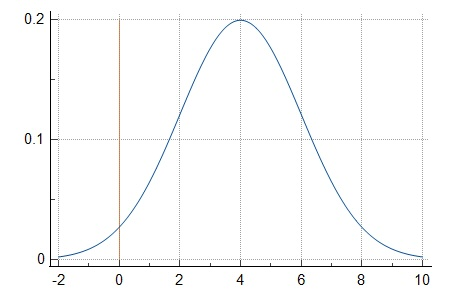
\includegraphics[width=.3\textwidth]{fig/fd_normal.jpg}}
	\raisebox{-0.5\height}{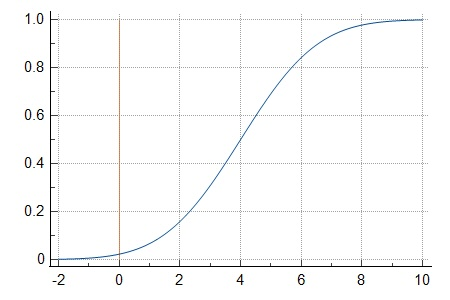
\includegraphics[width=.3\textwidth]{fig/fdpc_normal.jpg}} 
	$\stackrel{\mbox{\tiny\url{https://www.medcalc.org/}}}{N(\mu=2, \sigma=1)}$

\end{frame}



%%%%%%%%%%%%%%%%%%%%%%%%%%%%%%%%%%
%%%%%%%%%%%%%%%%%%%%%%%%%%%%%%%%%%
\begin{frame}{Distribuciones de Probabilidad  con Variables Continuas - II}

Consideremos $\mathbf{X}=(X_1, X_2, \ldots, X_n)$, $n$-variables continuas:

\begin{itemize}
\item Función de \key{distribución acumulada conjunta}:
    \begin{eqnarray*}
    F_{\mathbf{X}}(x_1, x_2, \ldots, x_n) & = & 
    		P(X_1 \leq x_1, X_2 \leq x_2, \ldots, X_n \leq x_n) \\
    		&=& \ds \int_{-\infty}^{x_1} \int_{-\infty}^{x_2} \cdots \int_{-\infty}^{x_n} f_{\mathbb{X}}(u_1, u_2, \ldots, u_n) \, du_n \, du_{n-1} \cdots du_1. 
    \end{eqnarray*}

\item Función de \key{densidad  conjunta}:
    $
    \ds f_{\mathbf{X}}(x_1, x_2, \ldots, x_n) = 
    \frac{\partial^n}{\partial x_1 \partial x_2 \cdots \partial x_n} F_{\mathbf{X}}(x_1, x_2, \ldots, x_n).
    $


\item Función de \key{distribución de probabilidad  conjunta}:
    $\ds P(\mathbf{X} \in \mathbf{A}) = \int_\mathbf{A} f_\mathbf{X}(\mathbf{x}) \, d\mathbf{x}$.

\item Función de \key{densidad de probabilidad  condicionada}: $f_{\mathbf{X}_{1\ldots k} \mid \mathbf{X}_{k+1\ldots n}}(\mathbf{x}_{1\ldots k} \mid \mathbf{x}_{k+1\ldots n})$\\
\hfil $
f_{X_1, X_2, \ldots, X_k \mid X_{k+1}, X_{k+2}, \ldots, X_n}(x_1, x_2, \ldots, x_k \mid x_{k+1}, x_{k+2}, \ldots, x_n) = 
\frac{f_{\mathbf{X}}(x_1, x_2, \ldots, x_n)}{f_{\mathbf{X}_{k+1\ldots n}}(x_{k+1}, x_{k+2}, \ldots, x_n)},
$

\item Función de \key{probabilidad condicionada}:\\
\small 
$\ds
P(\mathbf{X}_{1 \ldots k} \in A \mid X_{k+1} = x_{k+1}, X_{k+2} = x_{k+2}, \ldots, X_n = x_n) = 
\int_A f_{\mathbf{X}_{1\ldots k} \mid \mathbf{X}_{k+1\ldots n}}(\mathbf{x}_{1\ldots k} \mid \mathbf{x}_{k+1\ldots n}) \, dx_1 \, dx_2 \cdots dx_k.
$



\end{itemize}

\end{frame}  
   
   
   



%%%%%%%%%%%%%%%%%%%%%%%%%%%%%%%%%%
%%%%%%%%%%%%%%%%%%%%%%%%%%%%%%%%%%
\subsection{Procesos Estocásticos}


%%%%%%%%%%%%%%%%%%%%%%%%%%%%%%%%%%
%%%%%%%%%%%%%%%%%%%%%%%%%%%%%%%%%%

\begin{frame}{Representación Matemática con el Tiempo}
\begin{itemize}
	\item $X(w)$, v.a.,  asigna un número de forma atemporal.
    \item Podemos asignar diferentes números en \key{diferentes instantes} de tiempo $X(t, w)$, donde $t \in T$.
    \item $T$: Conjunto de \key{parámetros del proceso} (usualmente instantes de tiempo).
    \item \key{Si fijamos el tiempo} $t$, al valor $t_0$: $X(t_0,w)=X(w)$ es una \textbf{variable aleatoria}.
    \item \key{Si fijamos el evento} $w$, al valor $w_0$: $X(t, w_0)=X(t)$ es una \textbf{función real sobre el tiempo}.
\end{itemize}


    \begin{columns}
        \begin{column}{0.4\textwidth}
            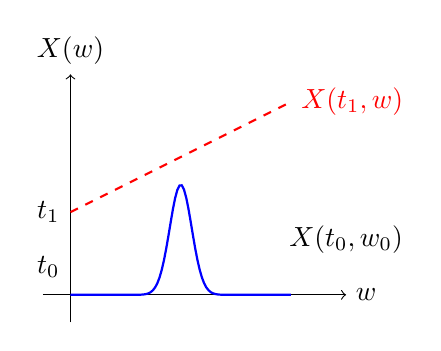
\begin{tikzpicture}[scale=.70]
                % Ejes
                \draw[->] (-0.5,0) -- (5,0) node[right] {$w$};
                \draw[->] (0,-0.5) -- (0,4) node[above] {$X(w)$};

    
                % Función X(w) para t_0
                % Función Normal N(0,1)
                \draw[blue, thick, domain=0:4, samples=100] 
                    plot (\x, {1/(0.2*sqrt(2*pi)) * exp(-(\x-2)*(\x-2)/(2*0.2*0.2))});
                \node at (5, 1) {$X(t_0, w_0)$};
                %\draw[thick,blue, dashed] plot[domain=0:4] (\x,{2 + 0.1*\x}) node[right] {$X(w, t_0)$};
                \node at (-0.4,0.5) {$t_0$};
                
                % Función X(w) para t_1
                \draw[thick,red,dashed] plot[domain=0:4] (\x,{1.5 + 0.5*\x}) node[right] {$X(t_1, w)$};
                \node at (-0.4,1.5) {$t_1$};
                               
            \end{tikzpicture}
            
            \textbf{\scriptsize Gráfica de \( X(w) \) para dos instantes temporales}
            
        \end{column}
        
        \begin{column}{0.4\textwidth}
            

            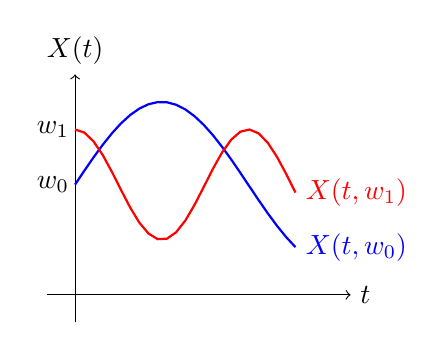
\begin{tikzpicture}[scale=.70]
                % Ejes
                \draw[->] (-0.5,0) -- (5,0) node[right] {$t$};
                \draw[->] (0,-0.5) -- (0,4) node[above] {$X(t)$};
                
                % Función X(t) para w_0
                \draw[thick,blue] plot[domain=0:4] (\x,{2 + 1.5*sin(\x r)}) node[right] {$X(t, w_0)$};
                \node at (-0.4,2) {$w_0$};
                
                % Función X(t) para w_1
                \draw[thick,red] plot[domain=0:4] (\x,{2 + 1.0*cos(2 * \x r)}) node[right] {$X(t, w_1)$};
                \node at (-0.4,3) {$w_1$};
         
            \end{tikzpicture}
            
            \textbf{\scriptsize Gráfica de \( X(t) \) para dos eventos}
        \end{column}
    \end{columns}

\end{frame}


%%%%%%%%%%%%%%%%%%%%%%%%%%%%%%%%%%
%%%%%%%%%%%%%%%%%%%%%%%%%%%%%%%%%%
\begin{frame}{Proceso Estocástico}

\begin{definition}[Proceso Estocástico]
Un \key{proceso estocástico} (PE) es una familia de variables aleatorias \(\{X(t)=X_t \mid t \in T\subseteq\mathbb{R} \}\) indexadas por un conjunto \(T\). 
\end{definition}

\begin{itemize}
\item \(T\) es un \key{conjunto de índices} que puede representar el tiempo (como \(\mathbb{R}_+\) o \(\mathbb{N}\)) o cualquier otro parámetro de interés.
\item \(X_t\) es una \key{variable aleatoria} para cada \(t \in T\).
\item Cada variable está definida sobre un \key{espacio de probabilidad} \((\Omega, \mathbb{B}, \mathbb{P})\), está compuesto por:
\begin{itemize}
    \item \(\Omega\): El \key{espacio muestral}, que es el conjunto de todos los posibles resultados del experimento.
    \item \(\mathbb{B}\): Una \key{\(\sigma\)-álgebra} sobre \(\Omega\), que es una colección de subconjuntos de \(\Omega\) sobre los cuales se pueden definir probabilidades.
    \item \(\mathbb{P}\): Una \key{medida de probabilidad} en \(\mathbb{B}\), que asigna probabilidades a los eventos en \(\mathcal{F}\).
\end{itemize}  

\item Los valores de $X(t, w)$ se llaman \key{estados}.
	\begin{itemize}
    \item El conjunto de valores constituye el \key{espacio de estados}, $S$.
    \end{itemize}
    

\item Un Proceso Estocástico estará descrito por sus \key{Funciones de Distribución} (de todo tipo). 

\begin{itemize}
\item Como $X_t$ es un v.a. para cada $t$, tiene sentido hablar de $F(x_i, t_i) = F(x_i) = P(X(t_i)\leq x_i)$ para cualquier  $t_i\in T$ arbitrario.
\item Así, podemos tener $n$ funciones: $F(x_1)$, $F(x_2)$, \ldots, $F(x_n)$ para $0\leq t_1 < t_2 < \cdots < t_n$.

\item Pero también tiene sentido hablar de \textbf{distribuciones conjuntas} $F(x_1, x_2, \ldots, x_n)$.

\end{itemize}

\end{itemize}
\end{frame}




 

%%%%%%%%%%%%%%%%%%%%%%%%%%%%%%%%%%
%%%%%%%%%%%%%%%%%%%%%%%%%%%%%%%%%%
\begin{frame}{Espacio Muestral vs Espacio de Estados}{Ejemplos de Procesos Estocásticos}

\begin{examples}
    \begin{enumerate}
        \item Lanzamiento de un dado ($T=\mathbb{Z}^+$)
        \begin{itemize}
        \item $\Omega = \{1, 2, 3, 4, 5, 6\}$  
        \item $S$ = \{par, impar\}
        \end{itemize}
        
        \item Temperatura diaria ($T=\mathbb{Z}^+$)
        \begin{itemize}
        \item $\Omega$ = \{Todos los posibles registros de temperatura para cada día del año\}
        \item $S$ = \{frío, templado, caluroso\}
        \end{itemize}
        
        \item Precio de una acción ($T=\mathbb{R}^+$)
        \begin{itemize}
        \item $\Omega$ = \{Todos los posibles precios de la acción (valores reales positivos)\}
		\item $S$ = \{subió, bajó, se mantuvo\}
		\end{itemize}
		
		\item Distancia entre 2 puntos en movimiento en un espacio bidimensional. ($T=\mathbb{R}^+$)
        \begin{itemize}
        \item $\Omega = \{(x_1, y_1, x_2, y_2) | (x_1, y_1)\in \mathbb{R}^2, (x_2, y_2)\in \mathbb{R}^2\}$
		\item $S = \{d| d\in[0,\infty)\}$ con $d=\sqrt{(x_2-x_1)^2+(y_2-y_1)^2}$
		\end{itemize}
		
		\item Piso en el que está un ascensor ($T=\mathbb{Z}^+$)
        \begin{itemize}
        \item $\Omega = \{(piso,$ \textit{\color{blue}dirección}$) | piso\in \{1, 2, \ldots, N\}, $\textit{\color{blue}dirección}$\in \{arriba, abajo, parado\}\}$
		\item $S = \{1, 2, \ldots, N\}$
		\end{itemize}	
				
    \end{enumerate}
\end{examples}
\end{frame}



%%%%%%%%%%%%%%%%%%%%%%%%%%%%%%%%%%
%%%%%%%%%%%%%%%%%%%%%%%%%%%%%%%%%%
\begin{frame}{Espacio Muestral vs Espacio de Estados}{Secuencias de Eventos}
En los ejemplos mostrados anteriormente se ha considerado que los elementos del espacio muestral son valores; pero pueden estar formados por secuencias de valores. 

\begin{examples}

\begin{itemize}
\item\key{Proceso de Bernoulli} modela situaciones donde obtenemos uno de dos posibles resultados  con una probabilidad fija para cada resultado.
	\begin{itemize}
	\item Espacio de estados: ${S}=\{0, 1\}$. 
	\item Espacio muestral: $\Omega=\{$Todas las posibles secuencias de $0$ y $1\}$
	
	\unEjemplo $\Omega=\{(0,1,0,1,...),(1,1,0,0,...),… \ldots \}$
	
	\begin{itemize}
	\item \textcolor{ejemplo}{Ejemplos de Procesos de Bernoulli}: \textbf{Inspección de Calidad} (determinar si cada artículo producido pasa o no). \textbf{Resultados de Exámenes Médicos} (seguimiento de resultados médicos repetidas para una enfermedad). \textbf{Resultados de Llamadas Telefónicas} (determinar si una llamada telefónica termina en venta), etc ...
	\end{itemize}
	
	\end{itemize}

	
\item\key{Proceso de Poisson} modela el nº de eventos en un intervalo de tiempo fijo $[0,T]$.
	\begin{itemize}
	\item Espacio de estados: $S=\mathbb{N}_0=\{0, 1, 2, \ldots\}$. Un valor representa el número de eventos.
	\item Espacio muestral: $\Omega=\{$Todas las posibles secuencias en $[0, T]\}$
	
	\unEjemplo $\Omega=\{(1),(4),\ldots, \underbrace{\ldots, (1, 3, 2), (0, 3, 1), \ldots}_{\mbox{\scriptsize Se hacen 3 lecturas}}, (1, 4, 2, 2), \ldots \}$
	
	\begin{itemize}
	\item \textcolor{ejemplo}{Ejemplos de Procesos de Poisson}: \textbf{Número de llamadas} que llegan a un central en un minuto, \textbf{número de clientes} por hora en una tienda, \textbf{número de fallos} de internet cada 15', \textbf{emisiones (nº) de partícula} en física nuclear,  etc ...
	\end{itemize}
	
	\end{itemize}
	

\end{itemize}

\end{examples}
\end{frame}




%%%%%%%%%%%%%%%%%%%%%%%%%%%%%%%%%%
%%%%%%%%%%%%%%%%%%%%%%%%%%%%%%%%%%

\subsection{Clasificación de los Procesos Estocásticos}



%%%%%%%%%%%%%%%%%%%%%%%%%%%%%%%%%%
%%%%%%%%%%%%%%%%%%%%%%%%%%%%%%%%%%

\begin{frame}{Clasificación de los Procesos Estocásticos}
    Los procesos estocásticos se clasifican de acuerdo a sus dos parámetros:
    \begin{itemize}
        \item \textbf{\color{reddark} Desde la perspectiva de $T$}:
        \begin{itemize}
            \item Si $T$ es un \textbf{intervalo de números reales} ($t$ toma valores continuos), el proceso estocástico se llama \key{de tiempo continuo}.
            \item Si $T$ es un conjunto \textbf{numerable} (y por tanto discreto), el proceso estocástico se llama \key{de tiempo discreto} o \key{secuencia aleatoria}. Se suele denotar $\{X[n]: n=1, 2,\ldots\}$.
        \end{itemize}
        
        \item \textbf{\color{reddark} Desde la perspectiva del conjunto de estados $S$}:
        \begin{itemize}
            \item Si $S$ es \textbf{continuo}, el proceso estocástico se llama \key{de estados continuos}.
            \item Si $S$ es \textbf{discreto}, el proceso se llama \key{de estados discretos}.
        \end{itemize}
    \end{itemize}

\vfill


\begin{tabularx}{\textwidth}{|c|X|X|}
    \hline
                      & $X$ \textbf{Discreto}                                      & $X$ \textbf{Continua}                                                \\ \hline
    \textbf{$t$ Discreto} & Proceso de estados discretos y tiempo discreto (\textbf{Cadena}) & Proceso de estados continuos y tiempo discreto        \\ \hline
    \textbf{$t$ Continuo} & Proceso de estados discretos y tiempo continuo (\textbf{Proc. Saltos Puros})    & Proceso de estados continuos y tiempo continuo (\textbf{Proceso Continuo})   \\ \hline
\end{tabularx}


\end{frame}


%%%%%%%%%%%%%%%%%%%%%%%%%%%%%%%%%%
%%%%%%%%%%%%%%%%%%%%%%%%%%%%%%%%%%
\subsubsection{Procesos de Markov}

%%%%%%%%%%%%%%%%%%%%%%%%%%%%%%%%%%
%%%%%%%%%%%%%%%%%%%%%%%%%%%%%%%%%%
\begin{frame}{Procesos de Markov}
\begin{itemize}
    \item Un proceso estocástico  se llama \key{Proceso de Markov de primer orden} si:
    \begin{eqnarray*}
     P(X(t_{n+1}) = x_{n+1}|X(t_n)=x_n, \ldots, X(t_1)=x_1) & = & P(X(t_{n+1}) = x_{n+1}|X(t_n)=x_n)\\
     P(\; \; X(t_{n+1}) \in A \; \;  |X(t_n)=x_n, \ldots, X(t_1)=x_1) & = & P(\; \; X(t_{n+1}) \in A \; \; |X(t_n)=x_n)
    \end{eqnarray*}
    \begin{itemize}
    \item \key{Propiedad de Markov:} dado el estado presente, el estado futuro es independiente del pasado.
    \end{itemize}
    
    \
    
    \item Un proceso estocástico se llama \key{Proceso de Markov de segundo orden} si:
    \begin{eqnarray*}
     P(X(t_{n+1}) = x_{n+1}|X(t_n)=x_n, \ldots, X(t_1)=x_1) & = & P(X(t_{n+1}) = x_{n+1}|X(t_n)=x_n, X(t_{n-1})=x_{n-1})\\
     P(\; \; X(t_{n+1}) \in A \; \;  |X(t_n)=x_n, \ldots, X(t_1)=x_1) & = & P(\; \; X(t_{n+1}) \in A \; \; |X(t_n)=x_n, X(t_{n-1})=x_{n-1})
    \end{eqnarray*}
    
    
    \item Y así sucesivamente ...
    
\end{itemize}

\end{frame}


%%%%%%%%%%%%%%%%%%%%%%%%%%%%%%%%%%
%%%%%%%%%%%%%%%%%%%%%%%%%%%%%%%%%%
\begin{frame}{Clasificación de Procesos de Markov}{Con algún ejemplo}

\begin{itemize}

\item \key{Clasificación de Procesos de Markov}
\begin{itemize}
    \item Desde la perspectiva del tiempo:
    \begin{itemize}
        \item Proceso de Markov de tiempo continuo vs de tiempo discreto.
    \end{itemize}
    \item Desde la perspectiva de los estados:
    \begin{itemize}
        \item Proceso de Markov de espacio de estados continuo vs de estados discreto.
    \end{itemize}
\end{itemize}


\item \key{Tipos de procesos de Markov según el tiempo y el espacio de estados:}

\hfil
\begin{tabularx}{.85\textwidth}{|l|X|X|}
\hline
                    & \textbf{Espacio de Estados, $X$, Discreto}           & \textbf{Espacio de Estados, $X$, Continuo}            \\ \hline
\textbf{Tiempo Discreto}  & Cadenas de Markov  & Procesos de Markov de estados continuos \\ \hline
\textbf{Tiempo Continuo}  & Proceso de Markov de tiempo continuo y estados discretos & Procesos de Markov continuo \\ \hline
\end{tabularx}

\begin{itemize}
\item
Salvo para la cadena de Markov, se suele especificar el tiempo de estados y de tiempo.
\end{itemize}

\item \key{Ejemplos de cada tipo de proceso de Markov:}


\hfil
\begin{tabularx}{.85\textwidth}{|l|X|X|}
\hline
                    & \textbf{Espacio de Estados, $X$, Discreto}           & \textbf{Espacio de Estados, $X$, Continuo}            \\ \hline
\textbf{Tiempo Discreto}  & Lanzamiento de moneda                      & Cantidad de lluvia caída cada mes               \\ \hline
\textbf{Tiempo Continuo}  & Número de clientes en la cola del supermercado & Velocidad del viento                          \\ \hline
\end{tabularx}

\end{itemize}
\end{frame}



%%%%%%%%%%%%%%%%%%%%%%%%%%%%%%%%%%
%%%%%%%%%%%%%%%%%%%%%%%%%%%%%%%%%%
\subsubsection{Cadenas de Markov}


%%%%%%%%%%%%%%%%%%%%%%%%%%%%%%%%%%
%%%%%%%%%%%%%%%%%%%%%%%%%%%%%%%%%%
\begin{frame}{Cadenas de Markov}
\begin{itemize}

\item 
\key{Proceso de Markov}: \textbf{proceso estocástico} $\{X_t\}_{t\in T}$, 
que es  \textbf{observable}, 
\underline{sin} \textbf{acciones} y 
que verifica la \textbf{Propiedad de Markov} (dado el estado presente, el estado futuro es independiente del pasado).

\item 
\key{Cadena de Markov:}  Proceso de Márkov tiene un \key{espacio de estados discreto} (numerable).


% - - - - - - - - CM en tiempos discretos
\item 
\key[red!80!black]{Cadena de Markov en tiempos discretos}, $t\in \mathbb{N}$    

\hfil $p_{ijn}=P\Big(X_n=s_j | X_{n-1} = s_i, \ldots, X_2=s_2, X_1=s_1\Big) = P\Big(X_n=s_j | X_{n-1} = s_i \Big)$

    \begin{itemize} 
      	
	\item 
	\key[ForestGreen]{Cadena Homogénea:} $p_{ijn}=p_{ij}$, es decir: 
		$P\Big(X_n=s_j | X_{n-1} = s_i \Big)=P\Big(X_1=s_j | X_{0} = s_i \Big)$ $\forall n, s_i, s_j$.
	
	\item 
	\key[ForestGreen]{Ecuaciones de Chapma-Kolmogorov:} Si $p_{ij}(n):=P(X_{n}=s_j|X_0=s_i)$, $P(n)=P^n=(\!(p_{ij})\!)^n$ entonces:\\
		\hfil $\ds \forall \; 0<r<n \; \; \; p_{ij}(n) = \sum_k p_{ik}(r) p_{kj}(n-r)$
		\hspace{0.5cm}
		$P(n+m)=P^{n+m}=P^nP^m=P(n)P(m)$. 
    \end{itemize}

% - - - - - - - - CM en tiempos continuos  
\item 
\key[red!80!black]{Cadena de Markov en tiempos continuos}, $t\in \mathbb{R}$

Para cada $t, t'\geq 0$ y  los correspondientes estados $s_i, s_j, \{s_{ku}|\ 0\leq u \leq t'\}$ se cumple:\\
\hfil $
p_{ij}(t', t'+t) = P\Big( X(t+t')=s_j | X(t') = s_i, X(u)=s_{k_u}, 0\leq u \leq t' \Big) = P\Big( X(t+t')=s_j|X(t')=s_i \Big) $

	\begin{itemize}
	\item 
	\key[ForestGreen]{Cadena homogénea:} $p_{ij}(t', t'+t)=p_{ij}(0, 0+t)=p_{ij}(t)$, es decir:

		\hfil $\ds p_{ij}(t)=P(X(t'+t)=s_j|X(t')=s_i)=P(X(t)=s_j|X(0)=s_i) \; \forall s_i, s_j\in S, t\geq 0 $


	\item 
	\key[ForestGreen]{Ecuaciones de Chapman-Kolmogorov:} 
		Si $\ds p_{ij}(t+s)= P\Big(X(t+s)=s_j| X(t)=s_i\Big)$\\
			\hfil $\ds p_{ij}(t+s)=\sum_k p_{ik}(t) p_{kj}(s) ; \forall s, t >0$ 
			\hspace{1cm}
			Si $P(t)=\Big(\!\!\Big(p_{ij}(t)\Big)\!\!\Big) \Rightarrow P(t+s)=P(t)P(s)$. 
	\end{itemize}


\end{itemize}

\end{frame}






%%%%%%%%%%%%%%%%%%%%%%%%%%%%%%%%%%
%%%%%%%%%%%%%%%%%%%%%%%%%%%%%%%%%%

\section{Construyendo un Proceso de Decisión de Markov en RL}






%%%%%%%%%%%%%%%%%%%%%%%%%%%%%%%%%%
%%%%%%%%%%%%%%%%%%%%%%%%%%%%%%%%%%

\subsection{La Interfaz Agente–Entorno}




%%%%%%%%%%%%%%%%%%%%%%%%%%%%%%%%%%
%%%%%%%%%%%%%%%%%%%%%%%%%%%%%%%%%%

\begin{frame}{La Interfaz Agente–Entorno}

\hfil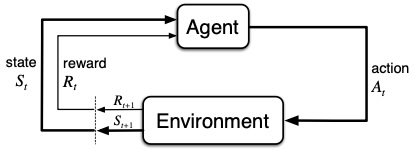
\includegraphics[width=0.5\textwidth]{fig/agent_environment_interaction}


\begin{itemize}
\item El agente y el entorno interactúa en una serie de \key{pasos} \( t = 0, 1, 2, 3, \ldots \).
\item En cada paso $t$:
	\begin{itemize}
	\item El agente recibe alguna representación del entorno (\key{estado}), $S_t\in \c{S}$
	\item El agente realiza una \key{acción} $A_t\in \c{A}(s)$ 
	\end{itemize}
\item En cada paso $t+1$, como consecuencia de la acción:
	\begin{itemize}
	\item El agente recibe una señal numérica (\key{recompensa}), $R_{t+1}\in \c{R}\subset \mbb{R}$
	\item El entono se encuentra en un \key{nuevo estado} $S_{t+1}$
	\end{itemize}

\item \key{Secuencia/Trayectoria}: $\c{H} \stackrel{\cdot}{=} S_0, A_0, R_1, S_1, A_1, R_2, S_2, A_2, R_3, \ldots$

\item Modelado: \key{PDM finito con recompensas}: $\c{S}$, $\c{A}$ y $\c{R}$ tiene un número finito de elemento.

%\item \key{Prob. Transición}: $p(s', r | s, a) \stackrel{\cdot}{=} \Pr\{S_t = s', R_t = r | S_{t-1} = s, A_{t-1} = a\}$
%
%\hfil$\sum_{s'} \sum_{r} p(s', r | s, a) = 1, \quad \text{para todo } s \in S, \ a \in A(s)$
%
%$p(s' | s, a) \stackrel{\cdot}{=} \Pr\{S_t = s' | S_{t-1} = s, A_{t-1} = a\} = \sum_{r \in R} p(s', r | s, a).$
\end{itemize}

\end{frame}





%%%%%%%%%%%%%%%%%%%%%%%%%%%%%%%%%%
%%%%%%%%%%%%%%%%%%%%%%%%%%%%%%%%%%
\subsection{Procesos de Markov}



%%%%%%%%%%%%%%%%%%%%%%%%%%%%%%%%%%
%%%%%%%%%%%%%%%%%%%%%%%%%%%%%%%%%%
\begin{frame}{Estados de Markov en RL}{Matriz de Transición de Estados}

\begin{itemize}
\item Definición formal. \key{Cadena de Markov en \underline{tiempos discretos}}, $t\in \mathbb{N}$    

\hfil $p_{ijn}=P\Big(X_n=s_j | X_{n-1} = s_i, \ldots, X_2=s_2, X_1=s_1\Big) = P\Big(X_n=s_j | X_{n-1} = s_i \Big)$



\item \key{Adaptamos a la notación del Aprendizaje por Refuerzo.}

\begin{itemize}
\item Un estado \( S_t \) es Markov si y solo si:
    \(
    Pr[S_{t+1} \mid S_t] = P[S_{t+1} \mid S_1, \dots, S_{t-1}, S_t]
    \)
    \begin{itemize}
        \item El estado captura toda la información relevante de la historia.
        \item Una vez conocido el estado, se puede descartar la historia.
    \end{itemize}
\end{itemize}

\item  Para un estado de Markov $s$ y un estado sucesor $s'$, la \key{probabilidad de transición }de estado se define por:
    \centerline{$p(s'|s) = P_{ss'} = Pr [S_{t+1} = s' | S_t = s]$}

\item La \key{matriz de transición de estados} $\mbf{P}$ define las probabilidades de transición de todos los estados $s$ a todos los estados sucesores $s'$:
    \begin{equation*}
        \mathbf{P} = \begin{bmatrix}
            P_{11} & \cdots & P_{1n} \\
            \vdots & \ddots & \vdots \\
            P_{n1} & \cdots & P_{nn}
        \end{bmatrix}
    \end{equation*}
    \begin{itemize}
   	\item $P_{ij}$ la probabilidad de transición partiendo del estado $i$ para llegar al estado $j$.
    \item Donde cada fila de la matriz suma 1.
	\end{itemize}

\end{itemize}

\end{frame}


%%%%%%%%%%%%%%%%%%%%%%%%%%%%%%%%%%
%%%%%%%%%%%%%%%%%%%%%%%%%%%%%%%%%%
\begin{frame}{Proceso (Cadena) de Markov}{Episodios}


\begin{definition}[Proceso de Markov]
	Un proceso de Markov es un proceso aleatorio sin memoria, es decir, 
	una secuencia de estados aleatorios $S_1, S_2, ...$ con la propiedad de Markov.
\end{definition}
    
\begin{definition}[Proceso de Markov]
    Un \key{Proceso de Markov} (o Cadena de Markov) es un par $\langle \c{S}, \mbf{P} \rangle$, donde:
    \begin{itemize}
        \item $\c{S}$ es un conjunto (finito) de estados.
        \item $\mbf{P}$ es una matriz de probabilidad de transición de estados, $p(s'|s)=P_{ss'} = P [S_{t+1} = s' | S_t = s]$.
    \end{itemize}
\end{definition}

\begin{definition}[Trayectoria/Episodio]
\begin{itemize}
\item Una \key{trayectoria} o historia de estados es una secuencia de estados.
\item Un \key{episodio} de estados es una historia que empieza en un estado inicial y finaliza es un estado terminal.
	\begin{itemize}
%	\item Estados no terminales: $\c{S}$
%	\item Todos los estados, más el terminal: $\c{S}^+$
	\item Un episodio es una muestra.
	\item Número de pasos: $T$ es una v.a. que depende del episodio.
	\end{itemize}
\end{itemize}
\end{definition}

\end{frame}



%%%%%%%%%%%%%%%%%%%%%%%%%%%%%%%%%%
%%%%%%%%%%%%%%%%%%%%%%%%%%%%%%%%%%
\begin{frame}{Ejemplo: Cadena de Markov del Estudiante}



\begin{columns}
\begin{column}{.6\textwidth}

\scalebox{.75}{
\begin{minipage}{\textwidth}
   \begin{tikzpicture}[
   		scale=0.8,
    	> = {Latex[width=8pt,length=8pt]},  % estilo de flecha
    	every path/.style = {line width=1pt}  % grosor para todos los paths
]
        \node[shape=ellipse, draw] (C1) at (0, 0) {$T_1$};
        \node[shape=ellipse, draw] (C2) at (4, 0) {$T_2$};
        \node[shape=ellipse, draw] (C3) at (8, 0) {$T_3$};
        \node[shape=ellipse, draw] (Pass) at (12, 0) {Superada};
        \node[shape=rectangle, draw] (Sleep) at (4, 3) {Dormir};
        \node[shape=ellipse, draw] (Red) at (0, 3) {Red};
        \node[shape=ellipse, draw] (Pub) at (3, -3) {Pub};

        \draw[->] (C1) -- node[above] {0.5} (C2);
        \draw[->] (C1) to[out=45,in=315] node[right] {0.5} (Red);
        
        \draw[->] (C2) -- node[above] {0.8} (C3);
        \draw[->] (C2) -- node[right] {0.2} (Sleep);
        
        \draw[->] (C3) -- node[above] {0.6} (Pass);
        \draw[->] (C3) to[out=270,in=0] node[right]  {0.4} (Pub);
        
        \draw[->] (Pass) to[out=90,in=0] node[below] {1.0} (Sleep);
		
        \draw[->] (Pub) -- node[left] {0.2} (C1);
        \draw[->] (Pub) -- node[left] {0.4} (C2);
        \draw[->] (Pub) -- node[left] {0.4} (C3);
        
        \draw[->] (Red) to[out=225,in=135] node[left] {0.1} (C1);
        \draw[->] (Red) to[out=45,in=135,looseness=8] node[above] {0.9} (Red);
    \end{tikzpicture}
\end{minipage}}


\end{column}
\begin{column}{.4\textwidth}
Episodios:
\begin{itemize}
\item $T_1$ $T_2$ $T_3$ Superada Dormir
\item $T_1$ Red Red $T_1$ $T_2$ Dormir
\item $T_1$ $T_2$ $T_3$ Pub $T_2$ $T_3$ Superada Dormir
\item $T_1$ Red Red $T_1$ $T_2$ $T_3$ Pub $T_1$ Red Red Red $T_1$ $T_2$ $T_3$ Pub $T_2$ Dormir
\end{itemize}
\end{column}
\end{columns}

\hfil{\footnotesize
\(\mathbf{P}=
\begin{blockarray}{cccccccc}
    & T_1 & T_2 & T_3 & \text{Superada} & \text{Pub} & \text{Red} & \text{Dormir} \\
\begin{block}{c[ccccccc]}
T_1      &     & 0.5 &     &            &          &  0.5     &       \\
T_2      &     &     & 0.8 &            &          &          &  0.2  \\
T_3      &     &     &     & 0.6        & 0.4      &          &       \\
\text{Superada} &     &     &     &            &          &          &  1    \\
\text{Pub}      & 0.2 &0.4  & 0.4 &            &          &          &       \\
\text{Red}      & 0.1 &     &     &            &          &  0.9     &       \\
\text{Dormir}    &     &     &     &            &          &          & 1     \\
\end{block}
\end{blockarray}
\)
}

\end{frame}




%%%%%%%%%%%%%%%%%%%%%%%%%%%%%%%%%%
%%%%%%%%%%%%%%%%%%%%%%%%%%%%%%%%%%

\subsection{Procesos de Recompensas de Markov}



%%%%%%%%%%%%%%%%%%%%%%%%%%%%%%%%%%
%%%%%%%%%%%%%%%%%%%%%%%%%%%%%%%%%%
\begin{frame}{Proceso de Recompensa de Markov (MRP)}


\begin{columns}
\begin{column}{.47\textwidth}

\begin{definition}[\key{Proceso de Recompensa de Markov}] 
Un MRP es un conjunto \( \langle \c{S}, \mbf{P}, {\color{reddark} \c{R}, \gamma } \rangle \), donde:
    \begin{itemize}
        \item \( \c{S} \): Conjunto finito de estados.
        \item \( \mbf{P} = (\!(p_{ss'})\!)\): Matriz de transición de estados. 
        
        {\color{reddark}
        \item \( \color{reddark} \c{R} = \{R_s | s\in \c{S}\} \subset \mbb{R}\): Recompensas finitas
        
        \( \color{reddark} R_s = r(s) = \mathbb{E}[R_{t+1} \mid S_t = s] \).
        
        \item \( \color{reddark} \gamma \): Factor de descuento (\( \color{reddark} \gamma \in [0, 1] \)).
        }
    \end{itemize}
\end{definition}



\begin{definition}[\key{Trayectoria/Episodio}]
\begin{itemize}
\item Una \textbf{trayectoria} o historia de estados es una secuencia de estados y recompensas.

\centerline{$S_0, R_1, S_1, R_2, S_2, \ldots $}
\item Un \textbf{episodio} es una historia que empieza en un estado inicial y finaliza en la recompensa del estado terminal

\centerline{$S_0, R_1, S_1, R_2, S_2, \ldots , S_T, R_T$}

\end{itemize}
\end{definition}



\end{column}

\begin{column}{.51\textwidth}

\begin{itemize}
\item Ejemplo: MRP del Estudiante
\end{itemize}

\scalebox{.6}{
\begin{minipage}{\textwidth}
   \begin{tikzpicture}[
   		scale=0.8,
    	> = {Latex[width=8pt,length=8pt]},  % estilo de flecha
    	every path/.style = {line width=1pt}  % grosor para todos los paths
		]
        \node[shape=ellipse, draw] (C1) at (0, 0) {$T_1$};
        \node at (1.25, -.4) {\color{reddark} R=-2}; % Cerca de T1 en el exterior
        
        \node[shape=ellipse, draw] (C2) at (4, 0) {$T_2$};
        \node at (5, -.40) {\color{reddark} R=-2};  % Cerca de T2 en el exterior
        
        \node[shape=ellipse, draw] (C3) at (8, 0) {$T_3$};
        \node at (9, -.40) {\color{reddark} R=-2};  % Cerca de T3 en el exterior
        
        \node[shape=ellipse, draw] (Pass) at (12, 0) {Superada};
        \node at (12, -0.7) {\color{reddark} R=+10};  % Cerca de Superada en el exterior
        
        \node[shape=rectangle, draw] (Sleep) at (4, 3) {Dormir};
        \node at (4, 3.70) {\color{reddark} R=0};  % Cerca de Dormir en el exterior
        
        \node[shape=ellipse, draw] (Red) at (0, 3) {Red};
        \node at (1.25, 2.6) {\color{reddark} R=-1}; % Cerca de Redes Sociales en el exterior
        
        \node[shape=ellipse, draw] (Pub) at (3, -3) {Pub};
        \node at (1.7, -3) {\color{reddark} R=+1}; % Cerca de BAR en el exterior
 

        \draw[->] (C1) -- node[above] {0.5} (C2);
        \draw[->] (C1) to[out=45,in=315] node[right] {0.5} (Red);
        
        \draw[->] (C2) -- node[above] {0.8} (C3);
        \draw[->] (C2) -- node[right] {0.2} (Sleep);
        
        \draw[->] (C3) -- node[above] {0.6} (Pass);
        \draw[->] (C3) to[out=270,in=0] node[right]  {0.4} (Pub);
        
        \draw[->] (Pass) to[out=90,in=0] node[below] {1.0} (Sleep);
		
        \draw[->] (Pub) -- node[left] {0.2} (C1);
        \draw[->] (Pub) -- node[left] {0.4} (C2);
        \draw[->] (Pub) -- node[left] {0.4} (C3);
        
        \draw[->] (Red) to[out=225,in=135] node[left] {0.1} (C1);
        \draw[->] (Red) to[out=45,in=135,looseness=8] node[above] {0.9} (Red);
    \end{tikzpicture}
\end{minipage}}

\begin{itemize}
    \item[] 
    \begin{itemize}
    \item $R_{T_1}=r_{T_2}=r_{T_3} = -2$
    \item $R_{Red}= -1$
    \item $R_{Pub}= +1$
    \item $R_{Superada}= +10$
    \item $R_{Dormir}=0$
    \end{itemize}
\end{itemize}


\end{column}
\end{columns}


\end{frame}



%%%%%%%%%%%%%%%%%%%%%%%%%%%%%%%%%%
%%%%%%%%%%%%%%%%%%%%%%%%%%%%%%%%%%
\begin{frame}{Recompensas y Retornos}
\begin{itemize}
\item \key{Recompensa Inmediata:} $R_s$, $R_{t}=R(S_t)$
\item \key{Función de recompensa:} $r(s)=\mathbb{E}[R_{t+1}|S_t=s]$
	\begin{itemize}
    	\item Para $t=0$, $r(s)=\mathbb{E}[R_{1}|S_t=s]$
    	\item Si entendemos que no se empieza en un estado concreto: $r(s)=R_s$
    	\item Si se interpreta como la recompensa esperad al salir del estado $s$: $r(s)=\sum_{s'} r_{s'} P_{ss'}$
	\end{itemize}

\item \key{Retorno} después del paso $t$: $\ds G_t=R_{t+1}+R_{t+2}+R_{t+3}+\cdots+R_T = \sum_{k=t+1}^{T} R_{k}$

\item \key{Retorno con descuento} después del paso $t$: $\ds G_t=R_{t+1} + \gamma R_{t+2} + \gamma^2 R_{t+3}+\cdots+ \gamma^{T-t-1} R_T=\sum_{k=t+1}^{T} \gamma^{k-t-1} R_{k}$ \textbf{para} \( \gamma \in[0,1] \).


\faForward{}  Motivos para \textbf{usar} un descuento:
    \begin{itemize}
        \item Representa la preferencia natural por recompensas inmediatas
        \item Refleja la incertidumbre del futuro
        \item Conveniencia matemática
        \item Evita retornos infinitos
    \end{itemize}

\faForward{}  Motivos para \textbf{no usar} un descuento ($\gamma = 1$):
	\begin{itemize}
	\item  Todas las trayectorias llevan a un estado terminal
	\end{itemize}
\end{itemize}
\end{frame}





%%%%%%%%%%%%%%%%%%%%%%%%%%%%%%%%%%
%%%%%%%%%%%%%%%%%%%%%%%%%%%%%%%%%%
\begin{frame}{Valores Esperados y Valores Esperados Condicionados}{Un repaso conceptual}
\begin{definition}[\key{Esperanza} / Expectativa / Valor esperado]
Dada una variable aleatoria $X$:
\begin{itemize}
\item Caso discreto. Dada $P[X=x]$, se define como $\ds \mbb{E} [X]=\sum _{x} x \operatorname {P} [X=x]$
\item Caso continuo. Dada $f_{X}(x)$, se define como $\ds\mbb{E} [X]= \int _{\mathbb {X} }x \cdot f_{X}(x)dx$.
\end{itemize}
\end{definition}

\begin{definition}[\key{Esperanza Condicional} (dado un valor)]
Dadas dos variables aleatorias $X$ e $Y$:
\begin{itemize}
\item Caso discreto. Dadas $P[X=x|Y=y]$, se define como $\ds \mbb{E} [X|Y=y]=\sum _{x} x \operatorname {P} [X=x|Y=y]$
\item Caso continuo. Dadas $f_{X|Y}(x|y)$, se define como $\ds\mbb{E} [X|Y=y]= \int _{\mathbb {X} } x \cdot f_{X|Y}(x|Y=y)dx$.
\end{itemize}
\end{definition}

\centerline{\Huge \texttwemoji{eye} \large \key{$\mbb{E}[X]$ es un número pero  $\mbb{E}[X|Y]$ es una variable aleatoria}}

\end{frame}




%%%%%%%%%%%%%%%%%%%%%%%%%%%%%%%%%%
%%%%%%%%%%%%%%%%%%%%%%%%%%%%%%%%%%
\begin{frame}{Expectativa Iterada}


\begin{theorem}[\key{Expectativas Iteradas} / Propiedad de las torres / Ley de la expectativa total ]
~\\
\centerline{\( \mathbb{E}[X] = \mathbb{E}[\mathbb{E}[X \mid Y]] \)}
\begin{itemize}
\item  \( X \) es una variable aleatoria.
\item  \( Y \) es una variable aleatoria \textbf{que afecta a la distribución de \( X \)}.
\end{itemize}

\end{theorem}

\begin{proof}
\begin{align*} \ds
\mathbb{E}_x[X] &  = \sum_x x P(X=x) = \sum_{y} \sum_{x} x P(X = x \mid Y = y) P(Y = y) \\
			  & = \sum_{y} \mathbb{E}_{x|y}[X \mid Y = y] P(Y = y) = \mathbb{E}_y[\mathbb{E}_{x|y}[X \mid Y]]
\end{align*}
\vskip -1.2cm ~ \hfill ~
\end{proof}

\vskip .5cm
\begin{example}[El retorno $\color{white} G_t$ a partir de un estado $\color{white} S_t$] 

~

Si $X=G_t$, $Y=S_t$ influye en $G_t$, entonces:
%
{\large \( \mathbb{E}[G_t] = \mathbb{E}[X] = \mathbb{E}[\, \mathbb{E}[X \mid Y] \, ] = \mathbb{E}[ \, \mathbb{E}[G_t \mid S_t] \, ] \quad \forall t\)}

~
\end{example}
\end{frame}





%%%%%%%%%%%%%%%%%%%%%%%%%%%%%%%%%%
%%%%%%%%%%%%%%%%%%%%%%%%%%%%%%%%%%
\begin{frame}{Función Valor}

\begin{definition}[Función Valor]
\key{Función valor de un estado}, $v(s)$, de un proceso de recompensas de Markov,
se define como:  \\[5pt]
\centerline{ {\large $v(s) = \mathbb{E}[G_t \mid S_t = s]$} con $\ds G_t = \sum_{k=0}^\infty \gamma^k R_{t+k+1}$}

\end{definition}


\begin{alertblock}{\faHandPointRight\/ Ecuaciones de Bellman}
~

\centerline{\Large ${\color{reddark}v(s)} = \mathbb{E}[R_{t+1} + \gamma {\color{reddark}v(S_{t+1})} \mid S_t = s]$}

~
\end{alertblock}

\begin{proof}
\begin{align*}
v(s) &= \mathbb{E}[G_t \mid S_t = s] = \mathbb{E}[R_{t+1} + \gamma R_{t+2} + \gamma^2 R_{t+3} + \dots \mid S_t = s] \\
     &= \mathbb{E}[R_{t+1} + \gamma (R_{t+2} + \gamma R_{t+3} + \dots) \mid S_t = s] = \mathbb{E}[R_{t+1} + \gamma G_{t+1} \mid S_t = s] \\
     &= \mathbb{E}[R_{t+1}\mid S_t = s] + \gamma {\color{red} \mathbb{E}[  G_{t+1} \mid S_t = s] }
      = \mathbb{E}[R_{t+1}\mid S_t = s] + \gamma {\color{red} \mathbb{E}[  \mathbb{E}[G_{t+1}|S_{t+1}] \mid S_t = s]} \\
     & = \mathbb{E}[R_{t+1}\mid S_t = s] + \gamma \mathbb{E}[ v(S_{t+1}) \mid S_t = s] \qquad \qquad \qquad \qquad {\color{aoenglish}\text{\faArrowAltCircleRight } \, \mathbb{E}[G_t] = \mathbb{E}[ \, \mathbb{E}[G_t \mid S_t] \, ] \forall t}
     \\
     &= \mathbb{E}[R_{t+1} + \gamma \cdot v(S_{t+1}) \mid S_t = s]
\end{align*}
\vskip -1.2cm ~ \hfill ~
\end{proof}

\vskip .5cm

\end{frame}





%%%%%%%%%%%%%%%%%%%%%%%%%%%%%%%%%%
%%%%%%%%%%%%%%%%%%%%%%%%%%%%%%%%%%
\begin{frame}{Resolución de las Ecuaciones de Bellman}

\scalebox{1.2}{
\begin{minipage}{.8\textwidth}
\begin{alertblock}{\faHandPointRight\/ Ecuaciones de Bellman}
~

\centerline{\large ${\color{reddark}v(s)} = \mathbb{E}[R_{t+1} + \gamma {\color{reddark}v(S_{t+1})} \mid S_t = s]$}

~
\end{alertblock}


\begin{itemize}
    \item La función de valor \key{se puede descomponer en dos partes}:
    \begin{itemize}
        \item Recompensa inmediata: $\mbb{E}[R_{t+1}|S_t=s]=R_s$
        \item Valor descontado del estado sucesor: $ \gamma\mbb{E}[v(S_{t+1})|S_t=s]= \gamma \sum_{s'} P_{ss'} v(s')$
    \end{itemize}
    \item \key{Nueva expresión:}
    $
    v(s) = R_s + \gamma \sum_{s'} P_{ss'} v(s')
    $
    
    
    \item \key{Forma matricial:}
    $
    \mbf{v} = \mbf{R} + \gamma \mbf{P} \cdot \mbf{v}
    $
    \hfill ¡¡ Responde a una ecuación lineal !!
    
    \item \key{Solución directa:}
    $\mbf{v} = \mbf{R} + \gamma \mbf{P} \cdot \mbf{v} \Rightarrow \mbf{Iv} = \mbf{R} + \gamma \mbf{P} \cdot \mbf{v}  \Rightarrow ( \mbf{I}-\gamma \mbf{P} ) \mbf{v} = \mbf{R} \Rightarrow$
    
    \centerline{\fbox{$\mbf{v} = (\mbf{I} - \gamma \mbf{P})^{-1} \mbf{R}$}}
    
    \begin{itemize}
    \item Complejidad computacional $O(n^3)$ para $n$ estados.
    
    \item No es la mejor solución. Hay métodos alternativos.
		
    \end{itemize}
    
\end{itemize}
\end{minipage}}

\end{frame}



%%%%%%%%%%%%%%%%%%%%%%%%%%%%%%%%%%
%%%%%%%%%%%%%%%%%%%%%%%%%%%%%%%%%%
\begin{frame}{Ejemplo: Cadena de Recompensas de Markov del Estudiante}
{Retornos Descontados  para un Episodio}


\hfil\scalebox{.75}{
\begin{minipage}{\textwidth}
   \begin{tikzpicture}[
   		scale=0.8,
    	> = {Latex[width=8pt,length=8pt]},  % estilo de flecha
    	every path/.style = {line width=1pt}  % grosor para todos los paths
		]
        \node[shape=ellipse, draw] (C1) at (0, 0) {$T_1$};
        \node at (1.25, -.4) {\color{reddark} R=-2}; % Cerca de T1 en el exterior
        
        \node[shape=ellipse, draw] (C2) at (4, 0) {$T_2$};
        \node at (5, -.40) {\color{reddark} R=-2};  % Cerca de T2 en el exterior
        
        \node[shape=ellipse, draw] (C3) at (8, 0) {$T_3$};
        \node at (9, -.40) {\color{reddark} R=-2};  % Cerca de T3 en el exterior
        
        \node[shape=ellipse, draw] (Pass) at (12, 0) {Superada};
        \node at (12, -0.7) {\color{reddark} R=+10};  % Cerca de Superada en el exterior
        
        \node[shape=rectangle, draw] (Sleep) at (4, 3) {Dormir};
        \node at (4, 3.70) {\color{reddark} R=0};  % Cerca de Dormir en el exterior
        
        \node[shape=ellipse, draw] (Red) at (0, 3) {Red};
        \node at (1.25, 2.6) {\color{reddark} R=-1}; % Cerca de Redes Sociales en el exterior
        
        \node[shape=ellipse, draw] (Pub) at (3, -3) {Pub};
        \node at (1.7, -3) {\color{reddark} R=+1}; % Cerca de BAR en el exterior
        
                                \node at (13, -3) {\Large $\ds G_0=R_{1}+\gamma R_{2}+ \gamma^2 R_{3}+\ldots \gamma^{T+1} R_T$};
 

        \draw[->] (C1) -- node[above] {0.5} (C2);
        \draw[->] (C1) to[out=45,in=315] node[right] {0.5} (Red);
        
        \draw[->] (C2) -- node[above] {0.8} (C3);
        \draw[->] (C2) -- node[right] {0.2} (Sleep);
        
        \draw[->] (C3) -- node[above] {0.6} (Pass);
        \draw[->] (C3) to[out=270,in=0] node[right]  {0.4} (Pub);
        
        \draw[->] (Pass) to[out=90,in=0] node[below] {1.0} (Sleep);
		
        \draw[->] (Pub) -- node[left] {0.2} (C1);
        \draw[->] (Pub) -- node[left] {0.4} (C2);
        \draw[->] (Pub) -- node[left] {0.4} (C3);
        
        \draw[->] (Red) to[out=225,in=135] node[left] {0.1} (C1);
        \draw[->] (Red) to[out=45,in=135,looseness=8] node[above] {0.9} (Red);
    \end{tikzpicture}
\end{minipage}}




\begin{columns}

\begin{column}{.4\textwidth}

\begin{itemize}
    \item[] 
    \begin{itemize}
    \item $R_{T_1}=r_{T_2}=r_{T_3} = -2$
    \item $R_{Red}= -1$
    \item $R_{Pub}= +1$
    \item $R_{Superada}= +10$
    \item $R_{Dormir}=0$
    \end{itemize}
\end{itemize}


\end{column}


\begin{column}{.6\textwidth}


\begin{itemize}
\item[] Para $\gamma=1/2$, algunos retornos empezando en $T_1$:


\begin{itemize}
\item $T_1$ $T_2$ $T_3$ Superada Dormir

$G_0 =  -2 - 2 \cdot \frac{1}{2} - 2 \cdot \frac{1}{4} + 10 \cdot \frac{1}{8} = -2.25$


\item $T_1$ Red Red $T_1$ $T_2$ Dormir

$G_0 = -2 - 1 \cdot \frac{1}{2} - 2 \cdot \frac{1}{4} - 1 \cdot \frac{1}{8} - 2 \cdot \frac{1}{16} = -3.125$


%\item $T_1$ $T_2$ $T_3$ Pub $T_2$ $T_3$ Superada Dormir
%
%$G_0 = -2 - 2 \cdot \frac{1}{2} - 2 \cdot \frac{1}{4} + 1 \cdot \frac{1}{8} - 2 \cdot \frac{1}{16} + \ldots = -3.41$
%
%\item $T_1$ Red Red $T_1$ $T_2$ $T_3$ Pub $T_1$ Red Red Red $T_1$ $T_2$ $T_3$ Pub $T_2$ Dormir
%
%$G_0 = -2 - 1 \cdot \frac{1}{2} - 2 \cdot \frac{1}{4} - 2 \cdot \frac{1}{8} - 2 \cdot \frac{1}{16} + \ldots = -3.20 $
\end{itemize}
\end{itemize}

\end{column}

\end{columns}

\end{frame}




%%%%%%%%%%%%%%%%%%%%%%%%%%%%%%%%%%
%%%%%%%%%%%%%%%%%%%%%%%%%%%%%%%%%%
\begin{frame}{Ejemplo: Cadena de Recompensas de Markov del Estudiante}
{Función de evaluación: Ecuaciones de Bellman}

\centerline{\large ${\color{reddark}v(s)} = \mathbb{E}[G_T|S_t=s]=\mathbb{E}[R_{t+1} + \gamma {\color{reddark}v(S_{t+1})} \mid S_t = s] = R_s + \gamma \sum_{s'} P_{ss'} v(s')$}

\begin{columns}

\begin{column}{.5\textwidth}


\scalebox{.6}{
\begin{minipage}{\textwidth}
   \begin{tikzpicture}[
   		scale=0.8,
    	> = {Latex[width=8pt,length=8pt]},  % estilo de flecha
    	every path/.style = {line width=1pt}  % grosor para todos los paths
		]
        \node[shape=ellipse, draw] (C1) at (0, 0) {\color{reddark} -5};
        \node at (1.25, -.4) {\color{aoenglish} R=-2}; % Cerca de T1 en el exterior
        
        \node[shape=ellipse, draw] (C2) at (4, 0) {\color{reddark} -.9};
        \node at (5, -.40) {\color{aoenglish} R=-2};  % Cerca de T2 en el exterior
        
        \node[shape=ellipse, draw] (C3) at (8, 0) {\color{reddark} -4.1};
        \node at (9, -.40) {\color{aoenglish} R=-2};  % Cerca de T3 en el exterior
        
        \node[shape=ellipse, draw] (Pass) at (12, 0) {\color{reddark} 10};
        \node at (12, -0.7) {\color{aoenglish} R=+10};  % Cerca de Superada en el exterior
        
        \node[shape=rectangle, draw] (Sleep) at (4, 3) {\color{reddark} 0};
        \node at (4, 3.70) {\color{aoenglish} R=0};  % Cerca de Dormir en el exterior
        
        \node[shape=ellipse, draw] (Red) at (0, 3) {\color{reddark} -7.6};
        \node at (1.25, 2.6) {\color{aoenglish} R=-1}; % Cerca de Redes Sociales en el exterior
        
        \node[shape=ellipse, draw] (Pub) at (3, -3) {\color{reddark} 1.9};
        \node at (1.7, -3) {\color{aoenglish} R=+1}; % Cerca de BAR en el exterior
 

        \draw[->] (C1) -- node[above] {0.5} (C2);
        \draw[->] (C1) to[out=45,in=315] node[right] {0.5} (Red);
        
        \draw[->] (C2) -- node[above] {0.8} (C3);
        \draw[->] (C2) -- node[right] {0.2} (Sleep);
        
        \draw[->, byzantine] (C3) -- node[above] {0.6} (Pass);
        \draw[->, byzantine] (C3) to[out=270,in=0] node[right]  {0.4} (Pub);
        
        \draw[->] (Pass) to[out=90,in=0] node[below] {1.0} (Sleep);
		
        \draw[->] (Pub) -- node[left] {0.2} (C1);
        \draw[->] (Pub) -- node[left] {0.4} (C2);
        \draw[->] (Pub) -- node[left] {0.4} (C3);
        
        \draw[->] (Red) to[out=225,in=135] node[left] {0.1} (C1);
        \draw[->] (Red) to[out=45,in=135,looseness=8] node[above] {0.9} (Red);
    \end{tikzpicture}
\end{minipage}}

\end{column}


\begin{column}{.5\textwidth}

\footnotesize
\begin{align*}
v(T_1) & = -2 + 0.9 \times (0.5 \cdot v(T_2) + 0.5 \cdot v(\text{Red})) \\
v(T_2) & = -2 + 0.9 \times (0.8 \cdot v(T_3) + 0.2 \cdot v(\text{Dormir})) \\
v(T_3) & = -2 + 0.9 \times ({\color{byzantine} 0.6} \cdot v(\text{Superada}) + {\color{byzantine}0.4} \cdot v(\text{Pub})) \\
v(\text{Red}) & = -1 + 0.9 \times (0.1 \cdot v(T_1) + 0.9 \cdot v(\text{Red})) \\
v(\text{Pub}) & = 1 + 0.9 \times (0.2 \cdot v(T_1) + 0.4 \cdot v(T_2) + 0.4 \cdot v(T_3)) \\
v(\text{Superada}) & = 10 + 0.9 \times v(\text{Dormir}) \\
v(\text{Dormir}) & = 0
\end{align*}


\begin{itemize}
\item A partir de $v(\text{Dormir}) = 0$ calculamos $v(\text{Superada})=10$
\item Y así vamos sustituyendo hasta resolver el sistema de ecuaciones.
\end{itemize}

\end{column}


\end{columns}

\end{frame}







%%%%%%%%%%%%%%%%%%%%%%%%%%%%%%%%%%
%%%%%%%%%%%%%%%%%%%%%%%%%%%%%%%%%%
\begin{frame}{Ejemplo: Cadena de Recompensas de Markov del Estudiante}
{Función de evaluación: Ecuaciones de Bellman con Resolución Matricial}

\centerline{\large $v(s) = R_s + \gamma \sum_{s'} P_{ss'} v(s') 
				\quad \Rightarrow \quad
				\mbf{v} = \mbf{R} + \gamma \mbf{P} \cdot \mbf{v}
				\quad \Rightarrow \quad$
				\fbox{$\color{reddark}  \mbf{v} = (\mbf{I} - \gamma \mbf{P})^{-1} \mbf{R}$}}

    
    
\begin{columns}

\begin{column}{.5\textwidth}



\scalebox{.6}{
\begin{minipage}{\textwidth}
   \begin{tikzpicture}[
   		scale=0.8,
    	> = {Latex[width=8pt,length=8pt]},  % estilo de flecha
    	every path/.style = {line width=1pt}  % grosor para todos los paths
		]
        \node[shape=ellipse, draw] (C1) at (0, 0) {\color{reddark} -5};
        \node at (1.25, -.4) {\color{aoenglish} R=-2}; % Cerca de T1 en el exterior
        
        \node[shape=ellipse, draw] (C2) at (4, 0) {\color{reddark} -.9};
        \node at (5, -.40) {\color{aoenglish} R=-2};  % Cerca de T2 en el exterior
        
        \node[shape=ellipse, draw] (C3) at (8, 0) {\color{reddark} -4.1};
        \node at (9, -.40) {\color{aoenglish} R=-2};  % Cerca de T3 en el exterior
        
        \node[shape=ellipse, draw] (Pass) at (12, 0) {\color{reddark} 10};
        \node at (12, -0.7) {\color{aoenglish} R=+10};  % Cerca de Superada en el exterior
        
        \node[shape=rectangle, draw] (Sleep) at (4, 3) {\color{reddark} 0};
        \node at (4, 3.70) {\color{aoenglish} R=0};  % Cerca de Dormir en el exterior
        
        \node[shape=ellipse, draw] (Red) at (0, 3) {\color{reddark} -7.6};
        \node at (1.25, 2.6) {\color{aoenglish} R=-1}; % Cerca de Redes Sociales en el exterior
        
        \node[shape=ellipse, draw] (Pub) at (3, -3) {\color{reddark} 1.9};
        \node at (1.7, -3) {\color{aoenglish} R=+1}; % Cerca de BAR en el exterior
 

        \draw[->] (C1) -- node[above] {0.5} (C2);
        \draw[->] (C1) to[out=45,in=315] node[right] {0.5} (Red);
        
        \draw[->] (C2) -- node[above] {0.8} (C3);
        \draw[->] (C2) -- node[right] {0.2} (Sleep);
        
        \draw[->] (C3) -- node[above] {0.6} (Pass);
        \draw[->] (C3) to[out=270,in=0] node[right]  {0.4} (Pub);
        
        \draw[->] (Pass) to[out=90,in=0] node[below] {1.0} (Sleep);
		
        \draw[->] (Pub) -- node[left] {0.2} (C1);
        \draw[->] (Pub) -- node[left] {0.4} (C2);
        \draw[->] (Pub) -- node[left] {0.4} (C3);
        
        \draw[->] (Red) to[out=225,in=135] node[left] {0.1} (C1);
        \draw[->] (Red) to[out=45,in=135,looseness=8] node[above] {0.9} (Red);
    \end{tikzpicture}
\end{minipage}}



\end{column}


\begin{column}{.5\textwidth}


\tiny
$
\begin{bmatrix}
v(T_1) \\
v(T_2) \\
v(T_3) \\
v(\text{Red}) \\
v(\text{Pub}) \\
v(\text{Superada}) \\
v(\text{Dormir})
\end{bmatrix}
=
\left(
\mathbf{I}
- \gamma
\begin{bmatrix}
0 & 0.5 & 0 & 0.5 & 0 & 0 & 0 \\
0 & 0 & 0.8 & 0 & 0 & 0 & 0.2 \\
0 & 0 & 0 & 0 & 0.4 & 0.6 & 0 \\
0.1 & 0 & 0 & 0.9 & 0 & 0 & 0 \\
0.2 & 0.4 & 0.4 & 0 & 0 & 0 & 0 \\
0 & 0 & 0 & 0 & 0 & 0 & 1 \\
0 & 0 & 0 & 0 & 0 & 0 & 0
\end{bmatrix}
\right)^{-1}
\cdot
\begin{bmatrix}
-2 \\
-2 \\
-2 \\
-1 \\
1 \\
10 \\
0
\end{bmatrix}
$

~

~

$
\begin{bmatrix}
v(T_1) \\
v(T_2) \\
v(T_3) \\
v(\text{Red}) \\
v(\text{Pub}) \\
v(\text{Superada}) \\
v(\text{Dormir})
\end{bmatrix}
=
\left(
\begin{bmatrix}
1.316 & 0.663 & 0.549 & 3.117 & 0.198 & 0.296 & 0.386 \\
0.079 & 1.160 & 0.959 & 0.187 & 0.345 & 0.518 & 0.675 \\
0.110 & 0.222 & 1.333 & 0.260 & 0.480 & 0.720 & 0.688 \\
0.623 & 0.314 & 0.260 & 6.740 & 0.094 & 0.140 & 0.183 \\
0.305 & 0.617 & 0.924 & 0.722 & 1.333 & 0.499 & 0.560 \\
0     & 0     & 0     & 0     & 0     & 1     & 0.9   \\
0     & 0     & 0     & 0     & 0     & 0     & 1
\end{bmatrix}
\right)
\cdot
\begin{bmatrix}
-2 \\
-2 \\
-2 \\
-1 \\
1 \\
10 \\
0
\end{bmatrix}
$

~

\scriptsize

\[
\mathbf{v} = \begin{bmatrix}
v(T_1) \\
v(T_2) \\
v(T_3) \\
v(\text{Red}) \\
v(\text{Pub}) \\
v(\text{Superada}) \\
v(\text{Dormir})
\end{bmatrix}
= \begin{bmatrix}
-5.01 \\
0.94 \\
4.08 \\
-7.63 \\
1.90 \\
10.0 \\
0
\end{bmatrix}
\qquad \text{ para } \gamma = 0.9\]



\end{column}


\end{columns}

\end{frame}





%%%%%%%%%%%%%%%%%%%%%%%%%%%%%%%%%%
%%%%%%%%%%%%%%%%%%%%%%%%%%%%%%%%%%

\subsection{Procesos de Decisión de Markov}


%%%%%%%%%%%%%%%%%%%%%%%%%%%%%%%%%%
%%%%%%%%%%%%%%%%%%%%%%%%%%%%%%%%%%
\begin{frame}{Procesos de Decisión de Markov (MDP)}




\begin{columns}
\begin{column}{.47\textwidth}

\begin{definition}[\key{Proceso de Decisión de Markov}] 
Un MDP es un conjunto \( \langle \c{S}, {\color{reddark} \c{A}}, \{\mbf{P}^{\color{reddark} a}\}_{\color{reddark} a}, \c{R}, \gamma  \rangle \), con:
\begin{itemize}
        \item \( \c{S} \): Conjunto finito de estados.
        \item \( {\color{reddark} \c{A} }\) \textcolor{reddark}{: Conjunto finito de acciones.}
        \item \( \mbf{P}^{\color{reddark} a} \): Matriz de transición de estados:
        
        \hfil\(
        P_{ss'}^{{\color{reddark}a}} = P(S_{t+1} = s' \mid S_t = s, {\color{reddark} A_t = a } )
        \)
        
        \item \( \c{R} \): Función de recompensa:
        \hfil\(
        R^{{\color{reddark}a}}_s =r(s,{\color{reddark} a})= \mathbb{E}[R_{t+1} \mid S_t = s, {\color{reddark} A_t = a}]
        \)
        
        \item \( \gamma \): Factor de descuento (\( \gamma \in [0, 1] \)).
\end{itemize}
\end{definition}



\begin{definition}[\key{Trayectoria/Episodio}]
\begin{itemize}
\item Una trayectoria o historia de estados es una secuencia de estados, acciones y recompensas.

\centerline{$S_0, A_0, R_1, S_1, A_1, R_2, S_2, A_2, R_3 \ldots $}

\end{itemize}
\end{definition}



\end{column}

\begin{column}{.51\textwidth}

\begin{itemize}
\item Ejemplo: MDP del Estudiante
\end{itemize}

\scalebox{.6}{
\begin{minipage}{\textwidth}
   \begin{tikzpicture}[
   		scale=0.8,
    	> = {Latex[width=8pt,length=8pt]},  % estilo de flecha
    	every path/.style = {line width=1pt}  % grosor para todos los paths
		]
        \node[shape=ellipse, draw] (C1) at (0, 0) {$T_1$};
        \node at (1.25, -.4) {\color{aoenglish} R=-2}; % Cerca de T1 en el exterior
        
        \node[shape=ellipse, draw] (C2) at (4, 0) {$T_2$};
        \node at (5, -.40) {\color{aoenglish} R=-2};  % Cerca de T2 en el exterior
        
        \node[shape=ellipse, draw] (C3) at (8, 0) {$T_3$};
        \node at (9, -.40) {\color{aoenglish} R=-2};  % Cerca de T3 en el exterior
        
        \node[shape=ellipse, draw] (Pass) at (12, 0) {Superada};
        \node at (12, -0.7) {\color{aoenglish} R=+10};  % Cerca de Superada en el exterior
        
        \node[shape=rectangle, draw] (Sleep) at (4, 3) {Dormir};
        \node at (4, 3.70) {\color{aoenglish} R=0};  % Cerca de Dormir en el exterior
        
        \node[shape=ellipse, draw] (Red) at (0, 3) {Red};
        \node at (1.25, 2.6) {\color{aoenglish} R=-1}; % Cerca de Redes Sociales en el exterior
        
        \node[circle, draw, fill=black, minimum size=5pt] (SobrePub) at (3, -3) {}; % Punto de decisión
        \node[right] at (SobrePub.east) {\color{reddark} \textbf{Volver}};
        
        \node[shape=ellipse, draw] (Pub) at (3, -5) {Pub};
        \node at (1.7, -5) {\color{aoenglish} R=+1}; % Cerca de BAR en el exterior
 

        \draw[->] (C1) -- node[above, yshift=2mm] {\color{reddark} Estudiar} 
        				  node[circle, draw, fill=black, scale=0.75, pos=0.5] {} (C2);
				  
        \draw[->] (C1) to[out=45,in=315] node[right,xshift=2mm] {\color{reddark} Móvil} 
        								 node[circle, draw, fill=black, scale=0.75, pos=0.5] {} (Red);
        
        \draw[->] (C2)  -- node[above, yshift=2mm] {\color{reddark} Estudiar} 
        				   node[circle, draw, fill=black, scale=0.75, pos=0.5] {} (C3);
				  
        \draw[->] (C2)  -- node[right, xshift=2mm] {\color{reddark} Descansar} 
        				   node[circle, draw, fill=black, scale=0.75, pos=0.45] {}  (Sleep);
        
        \draw[->] (C3)  -- node[above, yshift=2mm] {\color{reddark} Estudiar} 
        				   node[circle, draw, fill=black, scale=0.75, pos=0.45] {} (Pass);
				  
        \draw[->] (C3) to[out=270,in=0]  node[right, xshift=2mm]  {\color{reddark} Pub} 
        							     node[circle, draw, fill=black, scale=0.75, pos=0.5] {}  (Pub);
        
        \draw[->] (Pass) to[out=90, in=0] node[below, yshift=-2mm] {\color{reddark} Descansar} 
        								  node[circle, draw, fill=black, scale=0.75, pos=0.5] {} (Sleep);
		
		% node[below, yshift=-3mm, xshift=-3mm] {\Large \color{reddark} \textbf{Volver}}
		
		
		\draw[->] (Pub) -- (SobrePub);
		
        \draw[->] (SobrePub) -- node[left] {0.2} (C1);
        \draw[->] (SobrePub) -- node[left] {0.4} (C2);
        \draw[->] (SobrePub) -- node[left] {0.4} (C3);
        

        
        \draw[->] (Red) to[out=225,in=135] node[left, xshift=-2mm] {\color{reddark} Apagar} 
        								   node[circle, draw, fill=black, scale=0.75, pos=0.5] {} (C1);
								   
        \draw[->] (Red) to[out=45,in=135,looseness=8] node[above, yshift=2mm] {\color{reddark} Móvil}
        								 node[circle, draw, fill=black, scale=0.75, pos=0.5] {}  (Red);
    \end{tikzpicture}
\end{minipage}}

\begin{itemize}
    \item[] 
    \begin{itemize}
    \item Se cambian algunas las probabilidades por acciones concretas.
    \item Solo se ha dejado aleatoriedad en la acción Volver.
    \item Se podría hacer dejado aleatoriedad en cualquier estado del que salga más de 1 flecha.
    \end{itemize}
\end{itemize}


\end{column}
\end{columns}

\end{frame}




%%%%%%%%%%%%%%%%%%%%%%%%%%%%%%%%%%
%%%%%%%%%%%%%%%%%%%%%%%%%%%%%%%%%%
\begin{frame}{Políticas}
\begin{itemize}
    \item Una \key{política} \( \pi \) es una \textbf{distribución sobre acciones} dadas las condiciones del estado:\\
    \centerline{ \(    \pi(a \mid s) = P(A_t = a \mid S_t = s)     \) }
    
    
    
    \textit{Un ejemplo de política}, donde existen 3 posibles acciones para un estado es:
    $
    \pi(a|s) = \begin{cases}
        0.3 & \text{si } a = a_1 \\
        0.2 & \text{si } a = a_2 \\
        0.5 & \text{si } a = a_3
        \end{cases}
        $

    \item Las políticas en los MDPs:
    \begin{itemize}
        \item Dependientes del estado actual (\key{Markovianas}): $\pi(a|s)=P(A_t=a|H_t)$
        \item Independientes del tiempo (\key{estacionarias}): $\pi_t(a \mid s) = \pi(a \mid s) \quad \forall t. $ (Si se prefiere, para \( t > 0 \), \( A_t \sim \pi(\cdot \mid S_t) \)
        \item Si siempre se toma la misma decisión (\key{determinística}): $\pi(s)$
    \end{itemize}
    
    \item Dada una política en un Proceso de \key{Decisión} de Markov $\mathcal{M} = \langle \mathcal{S}, \mathcal{A}, \mbf{P}, \mathcal{R}, \gamma \rangle$ genera trayectorias $S_0, A_0, R_1, S_1, \ldots $
	Entonces, podemos definir:
    \begin{itemize}
    			
        \item Un proceso de \key{recompensa} de Markov $\langle \mathcal{S}, \mbf{P}^\pi, \mathcal{R}^\pi, \gamma \rangle$ (quitando acciones)
        	\begin{itemize}
			\item Genera la secuencia de estados y recompensas $S_0, R_1, S_1, \ldots$ 
			\end{itemize}
			
			
        \item Un \key{proceso} de Markov $\langle \mathcal{S}, \mbf{P}^\pi \rangle$ (quitando recompensas)
        	\begin{itemize}
			\item Genera la secuencia de estados $S_0, S_1, \ldots$ 
			\end{itemize}

        \item Donde: 
        \( P^\pi_{s, s'} = \ds \sum_{a \in \mathcal{A}} \pi(a \mid s) P^a_{s, s'} \)
        \qquad
        \( R^\pi_s = \ds \sum_{a \in \mathcal{A}} \pi(a \mid s) R^a_s \)
    
    
    \end{itemize}

    

\end{itemize}

\end{frame}


%%%%%%%%%%%%%%%%%%%%%%%%%%%%%%%%%%
%%%%%%%%%%%%%%%%%%%%%%%%%%%%%%%%%%
\begin{frame}{Ejemplo de PM y PRM a partir de un PDM}
\begin{itemize}
\item Proceso de Decisión de Markov con 2 acciones, 2 estados y 4 recompensas.

\begin{itemize}
\item Matriz de la políticas: \qquad \qquad \qquad \quad \,
 							 \(\pi(a|s) =
                                \begin{bmatrix}
                                \pi(a_1|s_1) & \pi(a_2|s_1) \\
                                \pi(a_1|s_2) & \pi(a_2|s_2)
                                \end{bmatrix}
                                \qquad\quad
                                =
                                \begin{bmatrix}
                                0.7 & 0.3 \\
                                0.4 & 0.6
                                \end{bmatrix}
                           \)

\item Matriz de transición (2 acciones): \qquad
							\(P(s'|s,a_1) =
                                \begin{bmatrix}
                                P(s_1|s_1,a_1) & P(s_2|s_1,a_1) \\
                                P(s_1|s_2,a_1) & P(s_2|s_2,a_1)
                                \end{bmatrix}
                                =
                                \begin{bmatrix}
                                0.5 & 0.5 \\
                                0.6 & 0.4
                                \end{bmatrix}
                            \)
                            
                            ~\qquad \qquad \qquad \qquad \qquad \qquad \qquad \,
                            \(
                            P(s'|s,a_2) =
                            \begin{bmatrix}
                            P(s_1|s_1,a_2) & P(s_2|s_1,a_2) \\
                            P(s_1|s_2,a_2) & P(s_2|s_2,a_2)
                            \end{bmatrix}
                            =
                            \begin{bmatrix}
                            0.2 & 0.8 \\
                            0.1 & 0.9
                            \end{bmatrix}
                            \)

\item Matriz de recompensas:  \qquad \qquad \qquad \quad \(R(s,a) = 
                            \begin{bmatrix}
                            R(s_1, a_1) & R(s_1, a_2) \\
                            R(s_2, a_1) & R(s_2, a_2)
                            \end{bmatrix}
                            \qquad
                            =
                            \begin{bmatrix}
                            10 & 5 \\
                            2 & 8
                            \end{bmatrix}
                            \)
\end{itemize}

\item Cálculo de \( P_{s,s'}^\pi =   \sum_{a \in \mathcal{A}} \pi(a \mid s) P(s' \mid s, a) \):

    \begin{itemize}
    \item \( P_{s_1,s_2}^\pi =   \sum_{a \in \mathcal{A}} \pi(a|s_1) P(s_2|s_1, a)\)
    	\begin{itemize}
    	\item Para \(a_1\): \(\pi(a_1|s_1) = 0.7\), \(P(s_2|s_1, a_1) = 0.5\).
    	\item Para \(a_2\): \(\pi(a_2|s_1) = 0.3\), \(P(s_2|s_1, a_2) = 0.8\).
    	\item Por tanto, $P_{s_1,s_2}^\pi = (0.7)(0.5) + (0.3)(0.8) = 0.35 + 0.24 = 0.59$
    	\end{itemize}
	\end{itemize}

\item Cálculo de $R_s^{\pi}  = \sum_{a \in \mathcal{A}} \pi(a \mid s) r(s, a) $
	\begin{itemize}
        \item \(  R_{s_1}^\pi = \sum_{a \in \mathcal{A}} \pi(a|s_1) R(s_1, a)\) 
        	\begin{itemize}
    		\item Para \(a_1\): \(\pi(a_1|s_1) = 0.7\), \(R(s_1, a_1) = 10\).
    		\item Para \(a_2\): \(\pi(a_2|s_1) = 0.3\), \(R(s_1, a_2) = 5\).
    		\item Por tanto, \(R_{s_1}^\pi = (0.7)(10) + (0.3)(5) = 7 + 1.5 = 8.5\)
    		\end{itemize}
	\end{itemize}
\end{itemize}


\TPMargin{0mm}%
\begin{textblock}{5.7}(10, 10) \small
\(
\mbf{P}^\pi = \begin{bmatrix}
P^\pi_{s_1,s_1} & P^\pi_{s_1,s_2} \\
P^\pi_{s_2,s_1} & P^\pi_{s_2,s_2}
\end{bmatrix} = 
\begin{bmatrix}
0.41 & 0.59 \\
0.3 & 0.7
\end{bmatrix}
\)
\end{textblock}

\TPMargin{0mm}%
\begin{textblock}{4.7}(10, 13.5) \small
\(
\mbf{R}^\pi = \begin{bmatrix}
R^\pi_{s_1} \\
R^\pi_{s_2}
\end{bmatrix} = 
\begin{bmatrix}
8.5 \\
5.6
\end{bmatrix}
\)
\end{textblock}

\end{frame}



%%%%%%%%%%%%%%%%%%%%%%%%%%%%%%%%%%
%%%%%%%%%%%%%%%%%%%%%%%%%%%%%%%%%%
\begin{frame}{Función Valor en un MDP}{Ecuaciones de Bellman}
\begin{itemize}
    \item La \key{función de valor de estado} \( v_\pi(s) \) es el retorno esperado desde el estado \( s \) siguiendo la política \( \pi \):
    \[
    v_\pi(s) = \mathbb{E}_\pi[G_t \mid S_t = s] 
    		 = \mathbb{E}_\pi \left[ \sum_{k=0}^\infty \gamma^k R_{t+k+1} \,\middle|\, S_t = s \right], 
		 		\quad \text{para todo } s \in \mathcal{S},
    \]
    
    \begin{itemize}
    \item \textbf{Ecuación de Bellman:}  \(\ds  v_\pi(s) = \mathbb{E}_\pi \left[ R_{t+1} + \gamma v_\pi(S_{t+1}) \mid S_t = s \right] \)
    \end{itemize}
    
    ~
    
    \item  La \key{función de valor estado-acció}n \( q_\pi(s, a) \) es el retorno esperado desde el estado \( s \), tomando la acción \( a \), y siguiendo la política \( \pi \):
    \[
    q_\pi(s, a) = \mathbb{E}_\pi[G_t \mid S_t = s, A_t = a] 
    		    = \mathbb{E}_\pi \left[ \sum_{k=0}^\infty \gamma^k R_{t+k+1} \,\middle|\, S_t = s, A_t=a\right], 
		 		\quad \text{para todos } s \in \mathcal{S},\, a\in \c{A}
    \]
    
	\begin{itemize}
    \item \textbf{Ecuación de Bellman:}  \(\ds  q_\pi(s, a) = \mathbb{E}_\pi \left[ R_{t+1} + \gamma q_\pi(S_{t+1}, A_{t+1}) \mid S_t = s, A_t = a \right] \)
    \end{itemize}
\end{itemize}

\end{frame}





%%%%%%%%%%%%%%%%%%%%%%%%%%%%%%%%%%
%%%%%%%%%%%%%%%%%%%%%%%%%%%%%%%%%%

\begin{frame}{Diagramas de Respaldo}

\begin{columns}
\begin{column}{.3\textwidth}
\begin{tikzpicture}[
	%scale=1.0,
	> = {Latex[width=4pt,length=8pt]},  % estilo de flecha
	%every path/.style = {line width=1pt}  % grosor para todos los paths
    state/.style={circle, draw, scale=10, inner sep=0},
    action/.style={circle, fill=black,  scale=5, inner sep=0},
    every node/.style={font=\scriptsize}
]

% Nodes
\node[state] (s) at (0,0) {};
\node (pi) at (0,-0.5) {$\pi(a|s)$};
\node[action] (a1) at (-1,-1) {};
\node[action] (a2) at (1,-1) {};
\node[state] (s11) at (-1.5,-2.2) {};
\node[state] (s12) at (-0.5,-2.2) {};
\node[state] (s21) at (0.5,-2.2) {};
\node[state] (s22) at (1.5,-2.2) {};



% Arrows
\draw[->] (s) -- (a1);
\draw[->] (s) -- (a2);

\draw[->] (a1) --  node[left, yshift=1mm] {$r$} (s11) ;
\draw[->] (a1) -- (s12);
\draw[->] (a2) -- (s21);
\draw[->] (a2) -- (s22);

% Additional labels
\node[left] at (s.west) {$s$};
\node[left] at (a1.west) {$a_1$};
\node[left] at (a2.west) {$a_2$};
\node[left] at (s11.west) {$s'$};


\end{tikzpicture}

\centerline{\tikz[remember picture] \node[coordinate] (inicio) {};}
\end{column}



\begin{column}{.3\textwidth}
\begin{tikzpicture}[
	%scale=1.0,
	> = {Latex[width=4pt,length=8pt]},  % estilo de flecha
	%every path/.style = {line width=1pt}  % grosor para todos los paths
    state/.style={circle, draw, scale=10, inner sep=0},
    action/.style={circle, fill=black,  scale=5, inner sep=0},
    every node/.style={font=\scriptsize}
]

% Nodes
\node[state] (s) at (0,0) {};
\node (pi) at (0,-0.5) {$\pi(a|s)$};
\node[action] (a1) at (-1,-1) {};
\node[action] (a2) at (1,-1) {};

% Arrows
\draw[->] (s) -- (a1);
\draw[->] (s) -- (a2);

% Additional labels
\node[left] at (s.west) {$v_\pi(s) \leftarrow s$};
\node[left] at (a1.west) {$q_\pi(s,a_1) \leftarrow s, a_1$};
\node[left] at (a2.west) {$a_2$};
\end{tikzpicture}


\end{column}



\begin{column}{.3\textwidth}
\begin{tikzpicture}[
	%scale=1.0,
	> = {Latex[width=4pt,length=8pt]},  % estilo de flecha
	%every path/.style = {line width=1pt}  % grosor para todos los paths
    state/.style={circle, draw, scale=10, inner sep=0},
    action/.style={circle, fill=black,  scale=5, inner sep=0},
    every node/.style={font=\scriptsize}
]

% Nodes
\node[action] (s) at (0,0) {};
\node[state] (a1) at (-1,-1) {};
\node[state] (a2) at (1,-1) {};




% Arrows
\draw[->] (s) --  node[left, yshift=1mm] {$r_1$} (a1);
\draw[->] (s) -- node[right, yshift=1mm] {$r_2$} (a2);


% Additional labels
\node[left] at (s.west) {$q_\pi(s,a) \leftarrow s,a$};
\node[left] at (a1.west) {$v_{\pi}(s'_1)\leftarrow s'_1$};
\node[left] at (a2.west) {$s'_2$};

\end{tikzpicture}



\end{column}


\end{columns}


~

$ $\hfill$v_\pi(s) = \sum_{a\in\c{A}} \pi(a|s) q_\pi(a,s)
\qquad 
q_\pi(s,a) = R^{a}_s + \gamma \sum_{s'\in\c{S}} P^{a}_{ss'} v_\pi(s')
$

~

~


\centerline{\text{\tikz[remember picture] \node[coordinate] (fin) {};}
$
v_\pi(s) = \sum_{a\in\c{A}} \pi(a|s) \left( R^{a}_s + \gamma \sum_{s'\in\c{S}} P^{a}_{ss'} v_\pi(s') \right)
$}


\begin{tikzpicture}[remember picture, overlay]
    \draw[->, thick, blue] (inicio) -- (fin);
\end{tikzpicture}

\end{frame}



%%%%%%%%%%%%%%%%%%%%%%%%%%%%%%%%%%
%%%%%%%%%%%%%%%%%%%%%%%%%%%%%%%%%%
\begin{frame}[t]{Cálculo de las Ecuación de Bellman}



\begin{columns}

\begin{column}{.5\textwidth}
\centering
\begin{tikzpicture}[
	scale=1.2,
	> = {Latex[width=4pt,length=8pt]},  % estilo de flecha
	%every path/.style = {line width=1pt}  % grosor para todos los paths
    state/.style={circle, draw, scale=10, inner sep=0},
    action/.style={circle, fill=black,  scale=5, inner sep=0},
    every node/.style={font=\scriptsize}
]

% Nodes
\node[state] (s) at (0,0) {};
\node (pi) at (0,-0.5) {$\pi(a|s)$};
\node[action] (a1) at (-1,-1) {};
\node[action] (a2) at (1,-1) {};
\node[state] (s11) at (-1.5,-2.2) {};
\node[state] (s12) at (-0.5,-2.2) {};
\node[state] (s21) at (0.5,-2.2) {};
\node[state] (s22) at (1.5,-2.2) {};



% Arrows
\draw[->] (s) -- (a1);
\draw[->] (s) -- (a2);

\draw[->] (a1) --  node[left, yshift=1mm] {$r$} (s11) ;
\draw[->] (a1) -- (s12);
\draw[->] (a2) -- (s21);
\draw[->] (a2) -- (s22);

% Additional labels
\node[left] at (s.west) {$v_\pi(s) \leftarrow s$};
\node[left] at (a1.west) {$q_\pi(s,a) \leftarrow s, a$};
\node[left] at (s11.west) {$v_\pi(s') \leftarrow s'$};

\end{tikzpicture}

\end{column}

\begin{column}{.5\textwidth}
\centering
\begin{tikzpicture}[
	scale=1.2,
	> = {Latex[width=4pt,length=8pt]},  % estilo de flecha
	%every path/.style = {line width=1pt}  % grosor para todos los paths
    state/.style={circle, draw, scale=10, inner sep=0},
    action/.style={circle, fill=black,  scale=5, inner sep=0},
    every node/.style={font=\scriptsize}
]

% Nodes
\node[action] (s) at (0,0) {};
\node[state] (a1) at (-1,-1) {};
\node (pi) at (-1.75,-1.5) {$\pi(a'|s')$};
\node[state] (a2) at (1,-1) {};
\node[action] (s11) at (-1.5,-2.2) {};
\node[action] (s12) at (-0.5,-2.2) {};
\node[action] (s21) at (0.5,-2.2) {};
\node[action] (s22) at (1.5,-2.2) {};



% Arrows
\draw[->] (s) --  node[left, yshift=1mm] {$r$} (a1);
\draw[->] (s) --  (a2);

\draw[->] (a1) --  (s11) ;
\draw[->] (a1) -- (s12);
\draw[->] (a2) -- (s21);
\draw[->] (a2) -- (s22);

% Additional labels
\node[left] at (s.west) {$q_\pi(s,a) \leftarrow s,a$};
\node[left] at (a1.west) {$s'$};
\node[left] at (s11.west) {$q_\pi(s', a') \leftarrow a'$};

\end{tikzpicture}

%{\small \( q_\pi(s, a) = \mathbb{E}_\pi[R_{t+1} + \gamma q_\pi(S_{t+1}, A_{t+1}) \mid S_t = s, A_t = a] \)}

\end{column}

\end{columns}

~

~

\vfill

\begin{itemize}
\item Para la función valor del estado:
    $$
    v_\pi(s) = \sum_{a\in\c{A}} \pi(a|s) \left( R^{a}_s + \gamma \sum_{s'\in\c{S}} P^{a}_{ss'} v_\pi(s') \right)
    $$

\item Para la función valor estado-acción:
    \[
    q_\pi(s, a) = R^a_s + \gamma \sum_{s' \in S} P^a_{ss'} \sum_{a' \in A} \pi(a' \mid s') q_\pi(s', a')
    \]
\end{itemize}

\end{frame}



%%%%%%%%%%%%%%%%%%%%%%%%%%%%%%%%%%
%%%%%%%%%%%%%%%%%%%%%%%%%%%%%%%%%%
\begin{frame}{Resolución Matricial}

\begin{itemize}
\item En un Proceso de \key{Recompensas} de Markov, con $P_{ss'}$:
	\begin{itemize}
	\item $\ds v(s) = R_s + \gamma \sum_{s'} P_{ss'} v(s')$
	\item \textbf{Forma matricial:} $\mbf{v} = \mbf{R} + \gamma \mbf{P} \cdot \mbf{v} $
		\begin{itemize}
		\item $\mbf{v}$ vector columna con valores $v(s)$ para todos los estados.
		\item $\mbf{R}$ vector columna con las recompensas $r(s)$ para todos los estados.
		\item $\mbf{P}= ((p_{ss'}))$, con las probabilidades de transición $p_{ss'}$.
		\end{itemize}
	\item Solución: $\mbf{v} = (\mbf{I} - \gamma \mbf{P})^{-1} \mbf{R}$ (si invertible)
	\end{itemize}
	
	
\item En un Proceso de \key{Decisión} de Markov, con $P_{ss'}^a$:
	\begin{itemize}
	\item $\ds v_\pi(s) = \sum_{a\in\c{A}} \pi(a|s) \left( R^{a}_s + \gamma \sum_{s'\in\c{S}} P^{a}_{ss'} v_\pi(s') \right) = \sum_{a\in\c{A}} \pi(a|s)  R^{a}_s + \gamma  \sum_{s'\in\c{S}} \sum_{a\in\c{A}} \pi(a|s) P^{a}_{ss'} v_\pi(s')  $
	\item \textbf{Forma matricial:} $\mbf{v}_\pi = \mbf{R}^\pi+ \gamma \mbf{P}^\pi \cdot \mbf{v}_\pi $
		\begin{itemize}
		\item $\mbf{v}_\pi$ vector columna con $v_\pi(s)$ para todos los estados. 
		\item $\mbf{R}^{\pi}$ vector columna con las recompensas esperadas $\ds \bar{r}_s^\pi = \sum_{a\in \c{A}} \pi(a|s) R_s^a$
		\item $\mbf{P}^{\pi}= ((\bar{p}_{ss'}^{\pi}))$ con las probabilidades esperadas $\ds \bar{p}_{ss'}^{\pi} = \sum_{a\in \c{A}} \pi(a|s) P_{ss'}^a$
		\end{itemize}
	\item Solución: $\mbf{v} = (\mbf{I} - \gamma \mbf{P}^\pi)^{-1} \mbf{R}^\pi$ (si invertible)
	\end{itemize}
	
	
\end{itemize}

\end{frame}


%%%%%%%%%%%%%%%%%%%%%%%%%%%%%%%%%%
%%%%%%%%%%%%%%%%%%%%%%%%%%%%%%%%%%
\subsection{PDM con Recompensas Estocásticas}



%%%%%%%%%%%%%%%%%%%%%%%%%%%%%%%%%%
%%%%%%%%%%%%%%%%%%%%%%%%%%%%%%%%%%
\begin{frame}{PDM con Recompensas Estocásticas}{Sutton \& Barto}

\centerline{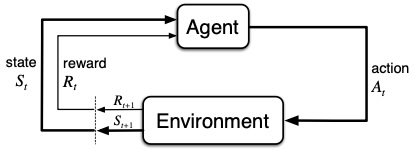
\includegraphics[width=0.5\textwidth]{fig/agent_environment_interaction}}


\begin{itemize}
\item \key{Trayectorias}: $S_0, A_0, R_1, S_1, A_1, R_2, S_2, A_2, R_3, \ldots$

\item \key{Transiciones}: Cambiamos $P^{a}_{ss'}$ por $P^{a{\color{reddark}r}}_{ss'}$. \textbf{\color{reddark} $\color{reddark} R_t$ es una v.a.}
	\begin{itemize}
	
	\item $P^{a{\color{reddark}r}}_{ss'}$: $p(s', {\color{reddark} r} | s, a) \stackrel{\cdot}{=} \Pr\{S_t = s', {\color{reddark} R_t = r} | S_{t-1} = s, A_{t-1} = a\}$ 
			con $\ds {\color{reddark} \sum_r}\sum_{s'}  p(s', {\color{reddark} r} | s, a) = 1$ 
			
	\item Podemos obtener $P^a_{ss'}$: $\ds p(s' | s, a) \stackrel{\cdot}{=} \Pr\{S_t = s' | S_{t-1} = s, A_{t-1} = a\} = \sum_{r \in R} p(s', r | s, a).$
	\end{itemize}

\item \key{Recompensas}:
	\begin{itemize}
	\item $\ds r(s, a) \stackrel{\cdot}{=} \mathbb{E}[R_t | S_{t-1} = s, A_{t-1} = a]  = \sum_{r \in R} r \cdot p(r | s, a) = \sum_{r \in R} r \sum_{s' \in S} p(s', r | s, a) = \sum_{r \in R} r \sum_{s' \in S} P^{ar}_{ss'} $
	\item $\ds r(s, a, s') \stackrel{\cdot}{=} \mathbb{E}[R_t | S_{t-1} = s, A_{t-1} = a, S_t = s']  = \sum_{r \in R} r \cdot p(r | s, a,s') = \sum_{r \in R} r \frac{p(s', r | s, a)}{p(s' | s, a)} = \sum_{r \in R} r.  \frac{P^{ar}_{ss'}}{P^a_{ss'}}   .$
	\end{itemize} 

\end{itemize}

\end{frame}





%%%%%%%%%%%%%%%%%%%%%%%%%%%%%%%%%%
%%%%%%%%%%%%%%%%%%%%%%%%%%%%%%%%%%
\begin{frame}{Función Valor en un MDP con Recompensas Estocásticas}{Ecuaciones de Bellman}
\begin{itemize}
    \item \key{Función  valor de estado:}\\
    \centerline{\(
    v_\pi(s) \stackrel{\cdot}{=} \mathbb{E}_\pi[G_t \mid S_t = s] \stackrel{Bellman}{=} \mathbb{E}_\pi[R_{t+1} + \gamma v_\pi(S_{t+1}) \mid S_t = s]
    \)}

    ~
    
    \item\key{ Función  valor estado-acción:}\\
    \centerline{
    \(
    q_\pi(s, a) \stackrel{\cdot}{=} \mathbb{E}_\pi[G_t \mid S_t = s, A_t = a]\stackrel{Bellman}{=} \mathbb{E}_\pi[R_{t+1} + \gamma q_\pi(S_{t+1}, A_{t+1}) \mid S_t = s, A_t = a]
    \)}

\end{itemize}

%\vskip1cm




\begin{block}{Diagramas de Respaldo}
\centerline{$\ds
v_\pi(s) = \sum_{a\in\c{A}} \pi(a|s) q_\pi(a,s)
\qquad%$}
%\centerline{$\ds
q_\pi(s,a) = {\color{reddark} \sum_{r\in\c{R}} r} \sum_{s'\in\c{S}} P^{a{\color{reddark} r}}_{ss'} + \gamma {\color{reddark} \sum_{r\in\c{R}}} \sum_{s'\in\c{S}} P^{a{\color{reddark} r}}_{ss'} v_\pi(s')
$}
\end{block}


\vskip -0.15cm

\begin{columns}

\begin{column}{.3\textwidth}
\begin{tikzpicture}[
	%scale=1.0,
	> = {Latex[width=4pt,length=8pt]},  % estilo de flecha
	%every path/.style = {line width=1pt}  % grosor para todos los paths
    state/.style={circle, draw, scale=10, inner sep=0},
    action/.style={circle, fill=black,  scale=5, inner sep=0},
    every node/.style={font=\scriptsize}
]

% Nodes
\node[state] (s) at (0,0) {};
\node (pi) at (0,-0.5) {$\pi(a|s)$};
\node[action] (a1) at (-1,-1) {};
\node[action] (a2) at (1,-1) {};

% Arrows
\draw[->] (s) -- node[inner sep=0, pos=0.5] (m1) {} (a1);
\draw[->] (s) -- node[inner sep=0, pos=0.5] (m2) {} (a2);



%\draw[thick]  (m1) to[out=-45, in=-125] (m2); % node[midway, below=5pt] {};
  
  
% Additional labels
\node[left] at (s.west) {$v_\pi(s) \leftarrow s$};
\node[left] at (a1.west) {$q_\pi(s,a) \leftarrow s, a$};
%\node[left] at (a2.west) {$a_2$};
\end{tikzpicture}


%\vskip1cm
\begin{tikzpicture}[
	%scale=1.0,
	> = {Latex[width=4pt,length=8pt]},  % estilo de flecha
	%every path/.style = {line width=1pt}  % grosor para todos los paths
    state/.style={circle, draw, scale=10, inner sep=0},
    action/.style={circle, fill=black,  scale=5, inner sep=0},
    every node/.style={font=\scriptsize}
]

% Nodes
\node[action] (s) at (0,0) {};
\node[state] (a1) at (-1,-1) {};
\node[state] (a2) at (1,-1) {};




% Arrows
\draw[->] (s) --  node[left, yshift=1mm] {$r$} (a1);
\draw[->] (s) -- node[right, yshift=1mm] {} (a2);


% Additional labels
\node[left] at (s.west) {$q_\pi(s,a) \leftarrow s,a$};
\node[left] at (a1.west) {$v_{\pi}(s')\leftarrow s'$};
%\node[left] at (a2.west) {$s'_2$};

\end{tikzpicture}
\end{column}


\begin{column}{.5\textwidth}
\begin{align*}
v_\pi(s)  & = \sum_{a\in\c{A}} \pi(a|s) \sum_{s',r} P_{ss'}^{ar} \left( r + \gamma v_\pi(s') \right) \\
q_\pi(s, a) & = \sum_{s',r} r \cdot P_{ss'}^{ar}  + \gamma \sum_{s', r} P^{ar}_{ss'} \sum_{a' \in \c{A}} \pi(a' \mid s') q_\pi(s', a') \\
& = \sum_{s',r}  P_{ss'}^{ar} \left( r  + \gamma  \sum_{a' \in \c{A}} \pi(a' \mid s') q_\pi(s', a') \right)
\end{align*}

\end{column}


\end{columns}


~

~

\end{frame}






%%%%%%%%%%%%%%%%%%%%%%%%%%%%%%%%%%
%%%%%%%%%%%%%%%%%%%%%%%%%%%%%%%%%%
\begin{frame}{Resolución Matricial}

\begin{itemize}
	\item En un Proceso de Decisión de Markov, con $P_{ss'}^a$:
	\begin{itemize}
	\item $\ds v_\pi(s) = \sum_{a\in\c{A}} \pi(a|s) \left( R^{a}_s + \gamma \sum_{s'\in\c{S}} P^{a}_{ss'} v_\pi(s') \right) = \sum_{a\in\c{A}} \pi(a|s)  R^{a}_s + \gamma  \sum_{s'\in\c{S}} \sum_{a\in\c{A}} \pi(a|s) P^{a}_{ss'} v_\pi(s')  $
	\item Forma matricial: $\mbf{v}_\pi = \mbf{R}^\pi+ \gamma \mbf{P}^\pi \cdot \mbf{v}_\pi $
		\begin{itemize}
		\item $\mbf{v}_\pi$ vector columna con $v_\pi(s)$ para todos los estados. 
		\item $\mbf{R}^{\pi}$ vector columna con las recompensas inmediatas esperadas $\ds \bar{r}_s^\pi = \sum_{a\in \c{A}} \pi(a|s) R_s^a$
		\item $\mbf{P}^{\pi}= ((\bar{p}_{ss'}^{\pi}))$ con las probabilidades esperadas $\ds \bar{p}_{ss'}^{\pi} = \sum_{a\in \c{A}} \pi(a|s) P_{ss'}^a$
		\end{itemize}
	\end{itemize}
	
\item $\ds v_\pi(s)   = \sum_{a\in\c{A}} \pi(a|s) \sum_{s',r} P_{ss'}^{ar} \left( R_s^a + \gamma v_\pi(s') \right)
 = \sum_{a\in\c{A}} \pi(a|s) \sum_{s',r} P_{ss'}^{ar} R_s^a +  \gamma \sum_{s'} \sum_{a\in\c{A}, r} \pi(a|s)   P_{ss'}^{ar} v_\pi(s')$
\begin{itemize}
	\item Forma matricial: $\mbf{v}_\pi = \mbf{R}^\pi+ \gamma \mbf{P}^\pi \cdot \mbf{v}_\pi $
		\begin{itemize}
		\item $\mbf{v}_\pi$ vector columna con $v_\pi(s)$ para todos los estados. 
		\item $\mbf{R}^{\pi}$ vector columna con las recompensas inmediatas esperadas $\ds R_s^\pi=\sum_{a\in\c{A}} \pi(a|s) \sum_{s',r} P_{ss'}^{ar} R_s^a = \sum_r p(r|s) R_s^a$
		\item $\mbf{P}^{\pi}= ((\bar{p}_{ss'}^{\pi})$ con las probabilidades esperadas de la transición $\ds \bar{p}_{ss'}^{\pi} = \sum_{a\in \c{A}} \pi(a|s) \sum_{r} P_{ss'}^{ar} =\sum_{a\in \c{A}} \pi(a|s) P_{ss'}^a$
		\end{itemize}
%	\item Solución: $\mbf{v} = (\mbf{I} - \gamma \mbf{P})^{-1} \mbf{R}$ (si invertible)
\end{itemize}

\item Solución: $\mbf{v_\pi} = (\mbf{I} - \gamma \mbf{P}^\pi)^{-1} \mbf{R}^\pi$ (si invertible)

\end{itemize}

\end{frame}


%%%%%%%%%%%%%%%%%%%%%%%%%%%%%%%%%%
%%%%%%%%%%%%%%%%%%%%%%%%%%%%%%%%%%
\subsection{El ejemplo del GridWorld}




%%%%%%%%%%%%%%%%%%%%%%%%%%%%%%%%%%
%%%%%%%%%%%%%%%%%%%%%%%%%%%%%%%%%%
\begin{frame}{Ejemplo: GridWorld}
\begin{columns}
\begin{column}{.5\textwidth}
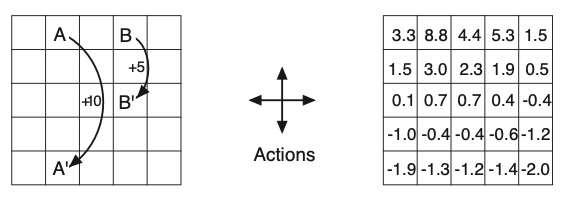
\includegraphics[width=\textwidth]{fig/gridworld_example}
\end{column}
\begin{column}{.45\textwidth}
\begin{itemize}
\item ¿Cuál es la ecuación de Bellman $v_\pi(A)$?
\item ¿Cuál es la ecuación de Bellman $v_\pi(A')$?
\item ¿Por qué hay valores negativos y positivos en los bordes?
\item ¿Por qué $v(A)<10$?
\item ¿Por qué $v(B)>5$?
\end{itemize}
\end{column}
\end{columns}


\begin{itemize}
\item Cada celda es un estado.
\item Se tienen 4 acciones en cada estado: norte, sur, este y oeste. Son equiprobables.
\item Estados futuros para cada acción: es determinístico. Dado por la acción.
\item Recompensas:  -1 si se sale del mundo. 0 en todos los demás.
	
\item Excepciones: 
	\begin{itemize}
	\item Si te sales del mundo vuelves al estado anterior.
	\item Si se sale de A se llega directamente a A' con recompensa +10.
	\item Si se sale de B se llega directamente a B' con recompensa +5.
	\end{itemize}
	
\item $\gamma = 0.9$ para la evaluación $v_{\pi}(s)$
\end{itemize}
%\end{itemize}

\end{frame}






%%%%%%%%%%%%%%%%%%%%%%%%%%%%%%%%%%
%%%%%%%%%%%%%%%%%%%%%%%%%%%%%%%%%%
\section{Políticas Óptimas}


%%%%%%%%%%%%%%%%%%%%%%%%%%%%%%%%%%
%%%%%%%%%%%%%%%%%%%%%%%%%%%%%%%%%%
\subsection{Optimalidad}

%%%%%%%%%%%%%%%%%%%%%%%%%%%%%%%%%%
%%%%%%%%%%%%%%%%%%%%%%%%%%%%%%%%%%
\begin{frame}{Funciones de Evaluación Óptimas y Políticas Optimas}

\begin{definition}[Funciones de Valor Óptimas]
\begin{itemize}
    \item \key{Función  valor de estado óptima:}
    
    	\centerline{$\ds v_*(s) \stackrel{\cdot}{=} \max_\pi v_\pi(s) \quad \forall s \in \c{S}$}
    
    \item \key{Función  valor de estado-acción óptima:}
    
		\centerline{$\ds q_*(s,a) \stackrel{\cdot}{=} \max_\pi q_\pi(s,a)  \quad \forall s \in \c{S}, \, \forall a \in \cal{A}$}
\end{itemize}


\begin{definition}[Ordenación (parcial) entre políticas]
\centerline{$ \pi \geq \pi' \text{ sii } v_\pi(s) \geq v_{\pi'}(s), \, \forall s $}
\end{definition}

\begin{theorem}[\textcolor{reddark}{Existencia de la Política Óptima}]
\begin{itemize}
\item  Para cualquier Proceso de Decisión de Markov \textbf{existe una política óptima} $\pi_*$ 
		verificando $\pi_*\geq \pi \quad \forall \pi$
\item Además $\ds v_*(s) = v_{\pi_*}(s)$ y $\ds q_*(s,a) = q_{\pi_*}(s,a)$
\end{itemize}
\end{theorem}


\end{definition}

\end{frame}




%%%%%%%%%%%%%%%%%%%%%%%%%%%%%%%%%
%%%%%%%%%%%%%%%%%%%%%%%%%%%%%%%%%
\begin{frame}{Ecuaciones de Bellman para Políticas Optimas}{Ecuaciones óptimas de Bellman}
  
\begin{description}
\item[\color{reddark}  Resultados Previos]

~\vskip-7mm ~
    \begin{align*} 
    \pi_*(a \mid s) & = 
\begin{cases} 
1 & \text{si } a = \arg\max\limits_{a \in \mathcal{A}} q_*(s, a), \\
0 & \text{de lo contrario}.
\end{cases} \\
    q_{\pi_*}(s,a) & \stackrel{\cdot}{=} \mbb{E}_{\pi_*}[G_t|S_t=s, A_t=a] \\
    			   & = \mbb{E}_{\pi_*} \left[R_{t+1} + \gamma G_{t+1} |S_t=s, A_t=a\right] \\
				   & = \mbb{E} \left[R_{t+1} + \gamma v_*(S_{t+1}) |S_t=s, A_t=a\right]  \quad \star
	\end{align*}  



\item [\color{reddark} Ecuación de Bellman Óptima para la Función de Valor de Estado]
    
    \begin{align*}
    v_*(s) & = \max_{a\in \c{A}(s)} q_*(s,a) = \max_{a\in \c{A}(s)} q_{\pi_*}(s,a) \\
		    & \stackrel{\star}{=} \max_a \mbb{E}[R_{t+1} + \gamma v_*(S_{t+1}) |S_t=s, A_t=a]
	\end{align*}

\item[\color{reddark} Ecuación de Bellman Óptima para la Función de Valor de Estado-Acción]
    
    \begin{align*}
    q_*(s,a) & \stackrel{\star}{=} \mbb{E}[R_{t+1} + \gamma v_*(S_{t+1}) |S_t=s, A_t=a] \\
    		& = \mbb{E}[R_{t+1}+ \gamma \max_{a'} q_* (S_{t+1}, a') |S_t=s, A_t=a]
	\end{align*}
	
\end{description}

\end{frame}



%%%%%%%%%%%%%%%%%%%%%%%%%%%%%%%%%%
%%%%%%%%%%%%%%%%%%%%%%%%%%%%%%%%%%
\begin{frame}{Cálculo de las Funciones de Valor Óptimas}

\begin{columns}

\begin{column}{.3\textwidth}
\begin{tikzpicture}[
	%scale=1.0,
	> = {Latex[width=4pt,length=8pt]},  % estilo de flecha
	%every path/.style = {line width=1pt}  % grosor para todos los paths
    state/.style={circle, draw, scale=10, inner sep=0},
    action/.style={circle, fill=black,  scale=5, inner sep=0},
    every node/.style={font=\scriptsize}
]

% Nodes
\node[state] (s) at (0,0) {};
\node (max) at (0,-0.25) {$\max$};
\node[action] (a1) at (-1,-1) {};
\node[action] (a2) at (1,-1) {};

% Arrows
\draw[->] (s) -- node[inner sep=0, pos=0.25] (m1) {} (a1);
\draw[->] (s) -- node[inner sep=0, pos=0.25] (m2) {} (a2);



\draw[thick]  (m1) to[out=-45, in=-125] (m2); % node[midway, below=5pt] {};
  
  
% Additional labels
\node[left] at (s.west) {$v_*(s) \leftarrow s$};
\node[left] at (a1.west) {$q_*(s,a) \leftarrow s, a$};
%\node[left] at (a2.west) {$a_2$};
\end{tikzpicture}
\end{column}


\begin{column}{.3\textwidth}
\begin{tikzpicture}[
	%scale=1.0,
	> = {Latex[width=4pt,length=8pt]},  % estilo de flecha
	%every path/.style = {line width=1pt}  % grosor para todos los paths
    state/.style={circle, draw, scale=10, inner sep=0},
    action/.style={circle, fill=black,  scale=5, inner sep=0},
    every node/.style={font=\scriptsize}
]

% Nodes
\node[action] (s) at (0,0) {};
\node[state] (a1) at (-1,-1) {};
\node[state] (a2) at (1,-1) {};




% Arrows
\draw[->] (s) --  node[left, yshift=1mm] {$r$} (a1);
\draw[->] (s) -- node[right, yshift=1mm] {} (a2);


% Additional labels
\node[left] at (s.west) {$q_*(s,a) \leftarrow s,a$};
\node[left] at (a1.west) {$v_*(s')\leftarrow s'$};
%\node[left] at (a2.west) {$s'_2$};

\end{tikzpicture}
\end{column}



\begin{column}{.4\textwidth}
\centerline{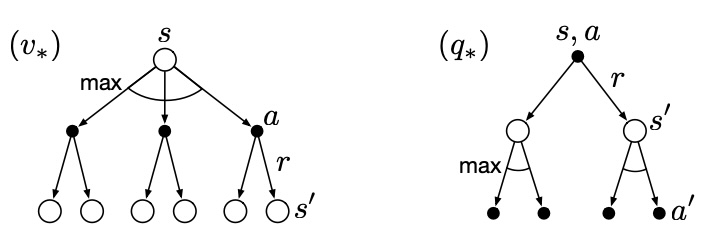
\includegraphics[width=\textwidth]{fig/backup_diagrams}}
\end{column}


\end{columns}


\begin{block}{PDM}
\centerline{$\ds 	v_*(s) = \max_a q_*(s,a) 
					\qquad \qquad \qquad
				 	q_*(s,a) = R_s^a + \gamma  \sum_{s'\in\c{S}} P^{a}_{ss'} v_*(s') 
		    $}
\centerline{$\ds 	v_*(s) = \max_a \left( R_s^a + \gamma  \sum_{s'\in\c{S}} P^{a}_{ss'} v_*(s') \right) 
					\qquad
				 	q_*(s,a) = R_s^a + \gamma  \sum_{s'\in\c{S}} P^{a}_{ss'}\max_a q_*(s,a) 
			$}
\end{block}




\begin{block}{PDM con Recompensas Estocásticas}
\centerline{$\ds 	v_*(s) = \max_a q_*(s,a) 
					\qquad \qquad \qquad \qquad \qquad
					q_*(s,a) = {\color{reddark} \sum_{r\in\c{R}} r} \sum_{s'\in\c{S}} P^{a{\color{reddark} r}}_{ss'} + 
								\gamma {\color{reddark} \sum_{r\in\c{R}}} \sum_{s'\in\c{S}} P^{a{\color{reddark} r}}_{ss'} v_*(s')
			$}
    \centerline{$\ds 	v_*(s) = \max_a \sum_{s', r} P_{ss'}^{ar} \left(r + \gamma v_*(s') \right] 
					\qquad \qquad \qquad
					q_*(s,a) = \sum_{s', r} P_{ss'}^{ar} \left( r + \gamma \max_{a'} q_*(s', a') \right)
			$}

\end{block}

\end{frame}

%%%%%%%%%%%%%%%%%%%%%%%%%%%%%%%%%%
%%%%%%%%%%%%%%%%%%%%%%%%%%%%%%%%%%
\begin{frame}{Resolviendo la Ecuación de Optimalidad de Bellman}
\scalebox{1.2}{
\begin{minipage}{.8\textwidth}
\begin{itemize}
	\item Las ecuaciones de optimalidad de Bellman no son lineales.
	\item \key{No existe una solución general} para las ecuaciones.
    \item \key{Métodos iterativos:}
    \begin{itemize}
        \item \textbf{Iteración del Valor}: Iteración sobre \( v(s) \) hasta convergencia.
        \item \textbf{Iteracion de la Política}: Alterna entre mejorar la política y evaluar \( v(s) \).
        \item \textbf{Q-learning}: Aproximación para encontrar \( q^*(s, a) \).
        \item \textbf{SARSA}
        \item etc ...
    \end{itemize}
     Estos métodos son fundamentales para resolver MDPs en la práctica y \key{definen las distintas técnicas del Aprendizaje por Refuerzo}.
\end{itemize}
\end{minipage}
}


\end{frame}






%%%%%%%%%%%%%%%%%%%%%%%%%%%%%%%%%%
%%%%%%%%%%%%%%%%%%%%%%%%%%%%%%%%%%
\subsection{El ejemplo del GridWorld}




%%%%%%%%%%%%%%%%%%%%%%%%%%%%%%%%%%
%%%%%%%%%%%%%%%%%%%%%%%%%%%%%%%%%%
\begin{frame}{Ejemplo: GridWorld}

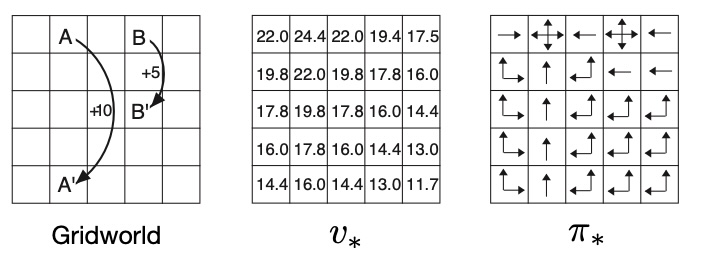
\includegraphics[width=\textwidth]{fig/optimalSolutionsGridworld}

\end{frame}




%%%%%%%%%%%%%%%%%%%%%%%%%%%%%%%%%%
%%%%%%%%%%%%%%%%%%%%%%%%%%%%%%%%%%
\section{Resumen}

%%%%%%%%%%%%%%%%%%%%%%%%%%%%%%%%%%
%%%%%%%%%%%%%%%%%%%%%%%%%%%%%%%%%%
\begin{frame}{Resumen para la \textcolor{reddark}{Función Valor de Estado}}

\begin{itemize}
\item \key{Definición:}
 \(\ds    v_\pi(s) = \mathbb{E}_\pi[G_t \mid S_t = s] 
    		 = \mathbb{E}_\pi \left[ \sum_{k=0}^\infty \gamma^k R_{t+k+1} \,\middle|\, S_t = s \right], 
		 		\quad \text{para todo } s \in \mathcal{S},
\)

\item \key{Ecuación de Bellman:} \(\ds  v_\pi(s) = \mathbb{E}_\pi \left[ R_{t+1} + \gamma v_\pi(S_{t+1}) \mid S_t = s \right] \)

    \begin{itemize}
    \item Proceso de \key{Decisión} de Markov
    
    \hfil $\ds
        v_\pi(s) = \sum_{a\in\c{A}} \pi(a|s) q_\pi(a,s) = \sum_{a\in\c{A}} \pi(a|s) \left( R^{a}_s + \gamma \sum_{s'\in\c{S}} P^{a}_{ss'} v_\pi(s') \right)
        $
    
    \item Proceso de Decisión de Markov con \key{Recompensas Estocásticas}
    
    \hfil $\ds
    v_\pi(s) = \sum_{a\in\c{A}} \pi(a|s) q_\pi(a,s) = \sum_{a\in\c{A}} \pi(a|s) \sum_{s',r} P_{ss'}^{ar} \left( r + \gamma v_\pi(s') \right) 
    $
    \end{itemize}

\item \key{Ecuación Óptima} de Bellman:
$\ds v_*(s)  = \max_{a\in \c{A}(s)} q_*(s,a) =  \max_a \mbb{E}[R_{t+1} + \gamma v_*(S_{t+1}) |S_t=s, A_t=a]$


    \begin{itemize}
    \item Proceso de \key{Decisión} de Markov
    
    \hfil $\ds v_*(s) = \max_a \left( R_s^a + \gamma  \sum_{s'\in\c{S}} P^{a}_{ss'} v_*(s') \right)$
    
    
    \item Proceso de Decisión de Markov con \key{Recompensas Estocásticas}
    
    \hfil $\ds v_*(s) = \max_a \sum_{s', r} P_{ss'}^{ar} \left(r + \gamma v_*(s') \right]$
    \end{itemize}
\end{itemize}

\end{frame}


%%%%%%%%%%%%%%%%%%%%%%%%%%%%%%%%%%
%%%%%%%%%%%%%%%%%%%%%%%%%%%%%%%%%%
\begin{frame}{Resumen para la \textcolor{reddark}{Función Valor de Estado-Acción}}

\begin{itemize}
\item \key{Definición: }
{\small $\ds
    q_\pi(s, a) = \mathbb{E}_\pi[G_t \mid S_t = s, A_t = a] 
    		    = \mathbb{E}_\pi \left[ \sum_{k=0}^\infty \gamma^k R_{t+k+1} \,\middle|\, S_t = s, A_t=a\right] 
		     \forall s \in \mathcal{S},\, \forall a\in \c{A}
    $}
    
\item  \key{Ecuación de Bellman:} 
$\ds  q_\pi(s, a) = \mathbb{E}_\pi \left[ R_{t+1} + \gamma q_\pi(S_{t+1}, A_{t+1}) \mid S_t = s, A_t = a \right]$


    \begin{itemize}
    \item Proceso de \key{Decisión} de Markov:
        
    \hfil$\ds   q_\pi(s, a) = R^{a}_s + \gamma \sum_{s'\in\c{S}} P^{a}_{ss'} v_\pi(s') 
    			= R^a_s + \gamma \sum_{s' \in S} P^a_{ss'} \sum_{a' \in A} \pi(a' \mid s') q_\pi(s', a')$
    
    \item Proceso de Decisión de Markov con \key{Recompensas Estocásticas}
    
    $\ds q_\pi(s,a) = {\color{reddark} \sum_{r\in\c{R}} r} \sum_{s'\in\c{S}} P^{a{\color{reddark} r}}_{ss'} + \gamma {\color{reddark} \sum_{r\in\c{R}}} \sum_{s'\in\c{S}} P^{a{\color{reddark} r}}_{ss'} v_\pi(s')
    = \sum_{s',r}  P_{ss'}^{ar} \left( r  + \gamma  \sum_{a' \in \c{A}} \pi(a' \mid s') q_\pi(s', a') \right)$
    \end{itemize}


\item \key{Ecuación Óptima} de Bellman:
$\ds q_*(s,a)= q_{\pi_*}(s,a) = \mbb{E}[R_{t+1}+ \gamma \max_{a'} q_* (S_{t+1}, a') |S_t=s, A_t=a] $


    \begin{itemize}
    \item Proceso de \key{Decisión} de Markov:
        
    \hfil$\ds  q_*(s,a) = R_s^a + \gamma  \sum_{s'\in\c{S}} P^{a}_{ss'}\max_a q_*(s,a)$
    
    \item Proceso de Decisión de Markov con \key{Recompensas Estocásticas:}
    
    \hfil $\ds q_*(s,a) = \sum_{s', r} P_{ss'}^{ar} \left( r + \gamma \max_{a'} q_*(s', a') \right)$
    \end{itemize}



\end{itemize}



\end{frame}






%%%%%%%%%%%%%%%%%%%%%%%%%%%%%%%%%%
%%%%%%%%%%%%%%%%%%%%%%%%%%%%%%%%%%
% BIBLIOGRAFÍA
%%%%%%%%%%%%%%%%%%%%%%%%%%%%%%%%%%
%%%%%%%%%%%%%%%%%%%%%%%%%%%%%%%%%%


%%%%%%%%%%%%%%%%%%%%%%%%%%%%%%%%%%%%%%%%%%%%%%%%%%%%%%%%%%%%%%%%%%%%
%%%%%%%%%%%%%%%%%%%%%%%%%%%%%%%%%%%%%%%%%%%%%%%%%%%%%%%%%%%%%%%%%%%%

\section{Referencias}



% Redefinimos la apariencia
%\setbeamertemplate{headline}{}
%\setbeamertemplate{frametitle}{\vskip 0.5cm	\small{\textbf{\insertframetitle}}}
%\setbeamertemplate{footline}{}




% Mostramos la bibliografía
% \begin{frame}[allowframebreaks] %% Si ocupa más de una página
%\begin{frame}[allowframebreaks]{Referencias -} %% Si hay sólo una página

\begin{frame}{Referencias} %% Si hay sólo una página
\nocite{Mausam2012, Russell2022, Sutton2018, silver2015, Hado2018Lecture}

	% \vskip -5cm %% Para ajustar la distancia al comienzo	
	%\bibliography{references}	
	\printbibliography[heading=none]
\end{frame}    


		
%%%%%%%%%%%%%%%%%%%%%%%%%%%%%%%%%%
%%%%%%%%%%%%%%%%%%%%%%%%%%%%%%%%%%

\end{document}

%%%%%%%%%%%%%%%%%%%%%%%%%%%%%%%%%%
%%%%%%%%%%%%%%%%%%%%%%%%%%%%%%%%%%